%% 
%% Copyright 2007, 2008, 2009 Elsevier Ltd
%% 
%% This file is part of the 'Elsarticle Bundle'.
%% ---------------------------------------------
%% 
%% It may be distributed under the conditions of the LaTeX Project Public
%% License, either version 1.2 of this license or (at your option) any
%% later version.  The latest version of this license is in
%%    http://www.latex-project.org/lppl.txt
%% and version 1.2 or later is part of all distributions of LaTeX
%% version 1999/12/01 or later.
%% 
%% The list of all files belonging to the 'Elsarticle Bundle' is
%% given in the file `manifest.txt'.
%% 

%% Template article for Elsevier's document class `elsarticle'
%% with numbered style bibliographic references
%% SP 2008/03/01

%\documentclass[preprint,12pt]{elsarticle}

%% Use the option review to obtain double line spacing
%% \documentclass[authoryear,preprint,review,12pt]{elsarticle}

%% Use the options 1p,twocolumn; 3p; 3p,twocolumn; 5p; or 5p,twocolumn
%% for a journal layout:
%% \documentclass[final,1p,times]{elsarticle}
%% \documentclass[final,1p,times,twocolumn]{elsarticle}
%% \documentclass[final,3p,times]{elsarticle}
%% \documentclass[final,3p,times,twocolumn]{elsarticle}
 \documentclass[final,5p,times]{elsarticle}
%% \documentclass[final,5p,times,twocolumn]{elsarticle}

%% For including figures, graphicx.sty has been loaded in
%% elsarticle.cls. If you prefer to use the old commands
%% please give \usepackage{epsfig}

%% The amssymb package provides various useful mathematical symbols
\usepackage{amssymb}
%% The amsthm package provides extended theorem environments
%% \usepackage{amsthm}

%% The lineno packages adds line numbers. Start line numbering with
%% \begin{linenumbers}, end it with \end{linenumbers}. Or switch it on
%% for the whole article with \linenumbers.
%% \usepackage{lineno}

\usepackage{algorithm}
\usepackage{algorithmic}

\journal{Parallel Computing}

\newif\ifdraft
%\drafttrue
\draftfalse
\ifdraft
 \newcommand{\eunsungnote}[1]{ {\textcolor{red}    { ***Eunsung:      #1 }}}
\else
 \newcommand{\eunsungnote}[1]{}
\fi

\begin{document}

\begin{frontmatter}

%% Title, authors and addresses

%% use the tnoteref command within \title for footnotes;
%% use the tnotetext command for theassociated footnote;
%% use the fnref command within \author or \address for footnotes;
%% use the fntext command for theassociated footnote;
%% use the corref command within \author for corresponding author footnotes;
%% use the cortext command for theassociated footnote;
%% use the ead command for the email address,
%% and the form \ead[url] for the home page:
%% \title{Title\tnoteref{label1}}
%% \tnotetext[label1]{}
%% \author{Name\corref{cor1}\fnref{label2}}
%% \ead{email address}
%% \ead[url]{home page}
%% \fntext[label2]{}
%% \cortext[cor1]{}
%% \address{Address\fnref{label3}}
%% \fntext[label3]{}

\title{Improving Sparse Data Movement Performance Using Multiple Paths on the Blue Gene/Q Supercomputer}

%% use optional labels to link authors explicitly to addresses:
%% \author[label1,label2]{}
%% \address[label1]{}
%% \address[label2]{}

\author[evl]{Huy Bui}
\author[mcs]{Eun-Sung Jung}
%\author[mcs]{Preeti Malakar}
\author[mcs]{Venkatram Vishwanath}
\author[evl]{Andrew Johnson}
\author[lava]{Jason Leigh}
\author[alcf,niu]{Michael E. Papka}

\address[evl]{Electronic Visualization Laboratory, University of Illinois at Chicago, 842 W. Taylor St., Chicago, IL 60607, USA}
\address[mcs]{Mathematics and Computer Science, Argonne National Laboratory, 9700 S. Cass Ave., Argonne, IL 60439, USA}
\address[alcf]{Argonne Leadership Computing Facility, Argonne National Laboratory, 9700 S. Cass Ave., Argonne, IL 60439, IL, USA}
\address[lava]{Laboratory for Advanced Visualization \& Applications (LAVA), University of Hawai'i at M{\~a}noa, 1680 East-West Road, Honolulu, HI 96822}
\address[niu]{Northern Illinois University, 300 Normal Road, DeKalb, IL 60115, USA}

\begin{abstract}

	In situ analysis has been proposed as a promising solution to glean faster insights and reduce the amount of data to storage. A critical challenge here is that the reduced dataset is typically located on a subset of the nodes and needs to be written out to storage. Data coupling in multiphysics codes also exhibits a sparse data movement pattern wherein data movement occurs among a subset of nodes. We evaluate the performance of data movement for sparse data patterns on the IBM Blue Gene/Q supercomputing system ``Mira'' and identify performance bottlenecks. We propose a multipath data movement algorithm for sparse data patterns based on an adaptation of a maximum flow algorithm together with breadth-first search that fully exploits all the underlying data paths and I/O nodes to improve data movement. We demonstrate the efficacy of our solutions through a set of microbenchmarks and application benchmarks on Mira scaling up to 131,072 compute cores. The results show that our approach achieves up to 5X improvement in achievable throughput compared with the default mechanisms.

\end{abstract}

\begin{keyword}
multiple paths \sep sparse data movement \sep topology-aware aggregation \sep data-intensive \sep Blue Gene/Q
%% keywords here, in the form: keyword \sep keyword

%% PACS codes here, in the form: \PACS code \sep code

%% MSC codes here, in the form: \MSC code \sep code
%% or \MSC[2008] code \sep code (2000 is the default)

\end{keyword}

\end{frontmatter}

%% \linenumbers

\section{Introduction}
Data-intensive applications generate large volumes of data. Data storage  performance is considered one of the weakest links in extreme-scale computing. In order to mitigate this I/O bottleneck, computational science applications are embracing in situ analysis and visualization wherein the analysis computation is performed at simulation time and a reduced dataset instead of the entire dataset
is written out to storage.
This approach helps reduce the amount of data being written to storage and allows users to glean scientific insights faster. Several in situ analyses, such as identification of regions of turbulence and query-driven analysis, produce sparse data, which needs to be written out to the storage system.
%GWP - WHY DOES IT NEED TO BE WRITTEN OUT? Almost immediately below you say that in many cases there may not be any data to write out!
Sparse data is characterized by having a wide distribution of message sizes for I/O across the compute nodes. In many cases,
because of the analyses performed and the data distribution,
a majority of nodes
may not have any data to write out to the storage system. This data movement pattern is called sparse in contrast to the dense data movement pattern, where data is evenly distributed among the compute nodes and data movement is carried out on a majority of compute nodes. 

Sparse data is also being generated by multiphysics applications, where different physics modules are running on disjoint compute partitions. Each module may write out data at different frequencies, probably non-overlapping, leading to a situation where the entire I/O pipeline may not be utilized to write the data from any single physics module. Furthermore, sparse data can be seen in communication between data coupling modules in multiphysics applications when one physics module needs data from another physics module to complete a computational task. The data is transferred between these modules through a single path, even though multiple paths are available for data transfer.

Since sparse data patterns are of increasing importance for computational science applications on leadership-class computers, optimizing and improving sparse data transfers on such systems are becoming more important.

In order to support higher bandwidth and to lower the messaging latency, interconnects in supercomputers are becoming more complex in terms of topology as well as routing policies. Currently various types of interconnect networks exist, such as the 3D torus in Cray XE6, 5D torus in Blue Gene/Q, 6D torus in K-machine, and Dragonfly in Cray XE30.  Leveraging all the available network paths is key to improved performance. Such network paths are not always fully exploited, however, because of application communication patterns and underlying routing policies. Current interconnects for supercomputers route a message along a single path. Different messages may have different paths depending on adaptive routing policies.
%GWP - It is not clear why having several options means restricting the paths - it seems better than one path. OR do you mean Nevertheless, such policies typically still route a message along one of the chosen paths, a reasonable strategy given the complexity of the interconnect networks ...
%GWP I also don't see why using only one path (assuming that with adaptive policies one still winds up doing only one path) is reasonable given the network complexity. If it is reasonable, however, does that make your porposed use of multiple paths unreasonable?
Adaptive routing gives several options to route data, resulting in only several paths to be selected. This is reasonable due to complexity of interconnect networks at scale under the assumption that all nodes carry on communication at a time. However, at user space, this leads to new opportunities for parallelizing message transfer and multi-path data movement for sparse data movement patterns.

In this paper, we propose a multipath data movement approach for sparse data patterns. Our approach is novel and practical in that it uses idle resources for handling sparse data movement through multiple paths. Moreover, it is implementable at the application level without needing modification of the underlying
hardware/software infrastructure. To our knowledge, our work is the first that proposes multipath data movement on the Blue Gene/Q (BG/Q) supercomputer for sparse data movement. More specifically, our contributions include the following.
\begin{itemize}
\item We adapt a max flow algorithm to find the possible number of disjoint paths to move data. 
We then use a breadth-first search (BFS) to find the paths. 
\item We realize multipath data movement by introducing intermediate nodes onto these paths. This approach overcomes the single-path data movement approach in the BG/Q under the current routing policy.
\item We leverage routing policies to reduce the number of intermediate nodes, in order to minimize overhead incurred by them.
\item In addition to multipath data movement, we implement pipelined data movement with the Parallel Active Message Interface (PAMI) library to further improve the data movement throughput.
\end{itemize}

The remainder of the paper is organized as follows. In Section \ref{sec:relatedwork} we present related work.
In Section \ref{sec:system}
we describe the IBM Blue Gene/Q system that we used in our study
In Section \ref{sec:approach}
we present our approach for multipaths data movement,
with the details of our algorithms and techniques to realize our ideas.
In Section \ref{sec:microbenchmark} and Section \ref{sec:appbenchmark} we demonstrate the efficacy of our solutions by using sets of microbenchmarks and application benchmarks, respectively.
In Section \ref{sec:conclusion}
we present our conclusions.

\section{Related work}
\label{sec:relatedwork}
Bandwidth optimization for data movement has been studied in great detail.
To optimize throughput, many researchers have considered a particular system's interconnection information and application's communication patterns. Essentially, these two characteristics can be used to map an application's processes to specific processors so that interprocessor communication can take advantage of that network to maximize throughput of data movement.

In an MPI-enabled environment, bandwidth optimization can be done via mapping the application's MPI processes to the system's processors/cores. In \cite{Bhatele:mapping}, the authors provided a tool for performing a wide variety of mappings for structured communication patterns. The mappings increased the bandwidth and reduced the latency and congestion. The tool did not take sparse communication patterns into account, however, and thus did not realize that multiple paths could be made available for data movement.

Kumar and Faraj \cite{Kumar:Allreduce} improved MPI\_Allreduce collective communication performance using multiple incoming and outgoing links per node communication on BG/Q. The work focused on MPI\_Allreduce collective communication, however, whereas our work targets sparse data movement among a subset of nodes.

Multipath data movement was established by Khanna et al. \cite{Proxies:Gaurav} by using intermediate nodes when an explicit path setup was not provided. This work focused on wide-area networks (WANs) where the exact network topology is hidden from users. Accordingly, shared links were identified through real experimental network throughput. In contrast, our work is applied to the interconnection network and the I/O subsystem of supercomputers where the network topology and associated routing policies are known a priori and the size of the network is much larger than that of WANs. Our ideas come from the observation that compute nodes in the BG/Q system have 10 links for communication but that usually only a single path is used for transferring data between nodes or between nodes and I/O nodes.

Adaptive routing for network load balancing has been also studied in \cite{Valiant:Routing,singh2003:goal}. 
In addition, researchers have investigated adaptive routing for current supercomputers such as  Blue Gene/Q \cite{Chen:BGQ} and Cray Cascade \cite{garcia2013:CrayDragonfly}. These studies are for low-level networking, however, where they are able to route any packet in any path. In contrast, our study leverages underlying routing policies to implement multipath data movement in the user space where we have more detailed knowledge about the data flows and the patterns. 
%More on load balancing network.

In the context of I/O forwarding and staging, many studies have been done to improve I/O performance.   
A scalable I/O forwarding framework for high-performance computing systems was presented in \cite{Ali:IOForwarding,Iskra:IOForwarding}. The authors in \cite{Vishwanath:IOForwarding,Vishwanath:GLEAN} proposed an augmentation for I/O forwarding and asynchronous data staging for Blue Gene/P and Blue Gene/Q systems, and the authors in \cite{ADIOS} proposed similar methods for Cray systems. However, those studies assumed that data is dense and uniformly distributed.

In our previous works in \cite{hbui:bgq, SDAV:Bui2014b, hbui:optiq} we focused on data movement for relatively dense communication patterns. Our work in this paper extends our previous work \cite{Vishwanath:GLEAN} to deal with sparse data movement patterns and extends our work in \cite{Multipath:BGQ} by employing a pipeline technique to reduce overhead and large memory usage caused by copying and injecting large messages. Our work also uses PAMI to improve the transfer of small messages.

\section{Systems for experiments}
\label{sec:system}

In this section, we describe the supercomputing systems in which we developed multipath sparse data movement algorithms and conducted our experiments. The Argonne Leadership Computing Facility (ALCF) maintains several compute-analysis systems used by the scientific community. Figure \ref{fig:alcf} depicts the architecture of the primary ALCF resources, consisting of the Blue Gene/Q compute cluster (Mira), the data analysis cluster (Tukey), and the file server nodes.

\begin{figure}[!htb]
\vspace{-0.1in}
\centering
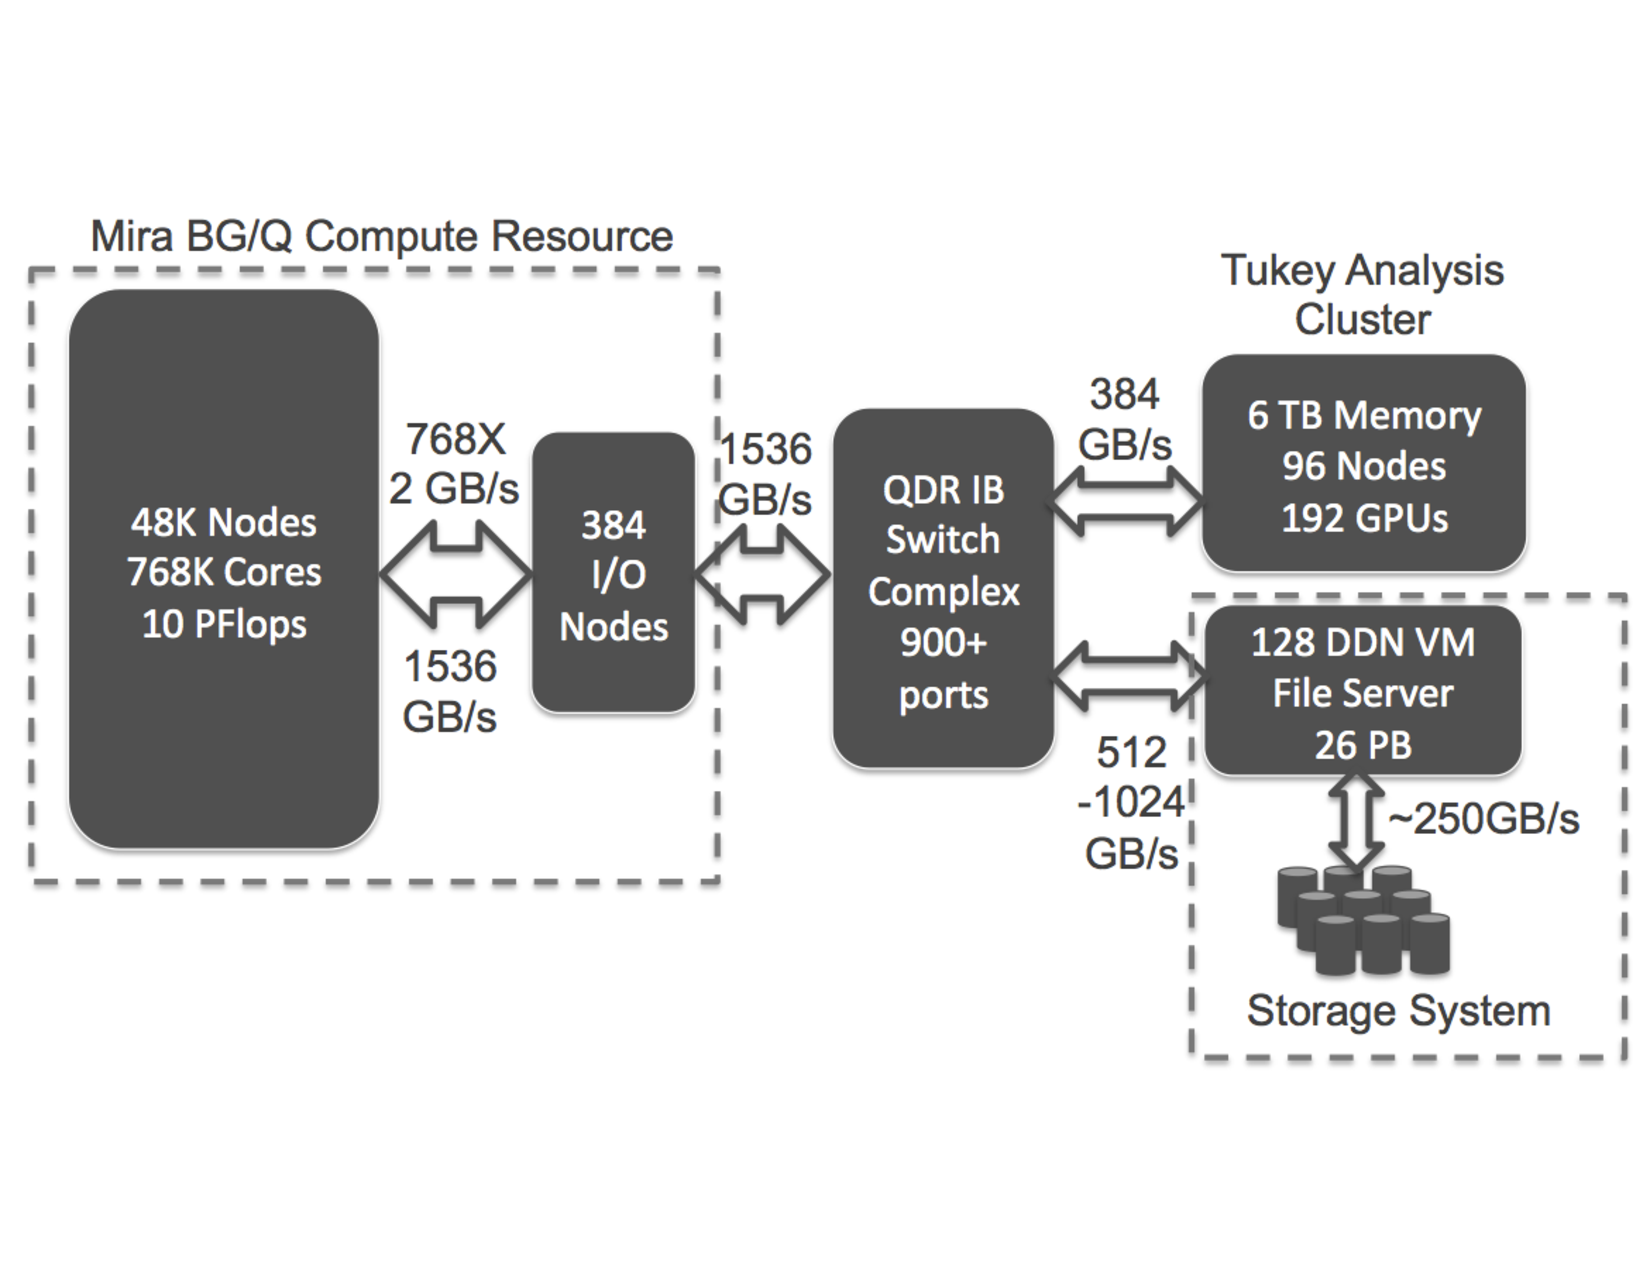
\includegraphics[scale=0.3]{anl_facility.pdf}
\vspace{-0.1in}
\caption{The ALCF maintains the 768K core Blue Gene/Q compute cluster (Mira), data analysis cluster (Tukey), and file server nodes.}
\vspace{-0.1in}
\label{fig:alcf}
\end{figure}


Mira \cite{Chen:BGQ}, with 48 compute racks (48K nodes and 768K cores) at the ALCF, provides 10 PFlops theoretical peak performance. Each node has a 16-core, 64-bit PowerPC A2 processor, together with 32 KB cached L1, 32 MB cache L2, and 16 GB of memory.

The I/O and interprocess communications of Blue Gene/Q travel on a 5D torus network both for point-to-point and for collective communications. This 5D torus interconnects a compute node with its 10 neighbors at 2 GB/s theoretical peak over each link in each direction, making a total of 40 GB/s bandwidth in both directions for a single compute node. Because of packet and protocol overheads, however, only up to 90\% of the raw data rate (1.8 GB/s) is available for user data. The machine can be partitioned into non-overlapping rectangular submachines; these submachines do not interfere with each other except for I/O nodes and the corresponding storage system.

For interconnect network traffic, BG/Q supports both deterministic and dynamic routing \cite{Chen:BGQ}. In deterministic routing, packets are routed based on dimension-ordered routing, from the longest first to the shortest last. In dynamic routing, routing is still dimension-ordered, but it is programmable, enabling different routing algorithms to be used. This approach is called ``zone routing.'' There are four zone ids, from 0 to 3. The routing algorithm selects a zone id based on the flexibility metric and message size. The flexibility value is computed based on the torus size and hop distance between two nodes doing communication. The selection of the zone id given the values is experiment-based and is hard coded in the low-level library \cite{BGQRedbook:Gilge}.
Routing zone id 0 is longest-to-shortest routing; however, dimensions with the same lengths can be chosen randomly. 
Routing zone id 1 is unrestricted routing, in which packets are routed in a random order.
Routing zone ids 2 and 3 are deterministic routing. For these two routing zone ids, given the size of a certain message, routing is always the same, and its path is known before it is routed. These are the default routing algorithms and cannot be changed during run time. However, one can set which routing zone id to use by using the PAMI\_ROUTING environment variable. Since BG/Q uses single-path data routing, for sending/receiving a message only one link of the ten available is used; hence, there is one reception FIFO at the receiver. In addition, for point-to-point communication, the number of hops between two nodes has negligible effect on performance.

On Mira, the compute nodes connect to an analysis cluster and file servers through I/O nodes and the QDR IB Switch Complex. Every 128 compute nodes (forming a pset) have two bridge nodes; two nodes in the pset have an additional functionality of a bridge node. Each bridge node has an 11th 2 GB/s bandwidth link connecting to an I/O node, making total 4 GB/s bandwidth for I/O per pset. I/O traffic is routed from the compute nodes to the bridge nodes over the torus network deterministically and then traverses over the 11th links from the bridge nodes to the I/O nodes.

PAMI is a low-level communication library for BG/Q \cite{PAMI:Kumar}. PAMI provides low-overhead communication by using various techniques such as accelerating communication using threads, scalable atomic primitives, and lockless algorithms to increase the messaging rate. Since MPI is implemented on top of PAMI, direct use of PAMI would provide higher messaging rates as well as lower latencies in comparison with MPI.


\section{Approach}
\label{sec:approach}
In this section, we present our multipath approach for sparse data movement in the leadership systems. We are able to use multiple paths for data movement through intermediate nodes called proxies while conforming to default routing policy enforced by the underlying infrastructure. We find multiple paths by adapting the maximum flow algorithm on the graph representing an interconnect network. We then improve performance by implementing pipeline techniques and using the PAMI low-level communication library.

We start by describing the inefficiencies of sparse data movement in the current systems. To overcome such inefficiencies, we propose novel approaches based on multipaths for sparse data movement.

\subsection{Inefficiency in current data movement}
For data transfer between compute nodes on BG/Q, a message traverses from a source to a destination node using a single path. In the absence of congestion and network failures, the default routing algorithm forces the message to traverse a deterministic single path. Figure \ref{fig:multiply}(a) depicts the single-path data movement, in which one path is used while the other paths are idle. With dense, uniform data movement patterns where the majority of nodes and network links involve communications, the utilization of system resources is high. With sparse data movement patterns, however, only specific regions of the system involve communications, resulting in a low utilization of the allocated resources.

Similarly, I/O messages (e.g., writes) from a compute node travel along a single path to a default I/O node, as shown in Figure \ref{fig:multiply}(b). When the writes  have a uniform distribution of data size and location, I/O nodes allocated for applications are used efficiently. With sparse data movements, however, I/O nodes and interconnect networks suffer from an unbalanced load. Current MPI-IO aggregates data into intermediate nodes, but these nodes are neither uniformly distributed nor balanced among all I/O nodes.

We next present a general approach to improve resource utilization for data movement. We then present our approach for sparse data movements.

\subsection{Data movement using multiple paths}
One way to improve the utilization is to employ multiple paths.
%To employ multiple path, 
We can assign multiple routing paths for multiple messages from a node. Theoretically, multiple messages would concurrently follow multiple non-overlapping paths, 
and the data movement therefore would achieve multifold improvement. At the programming level, however, the BG/Q supercomputer does not allow paths for messages to be set up explicitly. Nevertheless, we can still implement concurrent data movements via multiple paths in user space by using proxies while following disclosed default routing policies. Doing so greatly simplifies the deployment of our heuristics and provides us with valuable validation and feedback for our approaches.

\begin{figure}[!htb]
\vspace{-0.1in}
\centering
\hspace*{-0.4cm}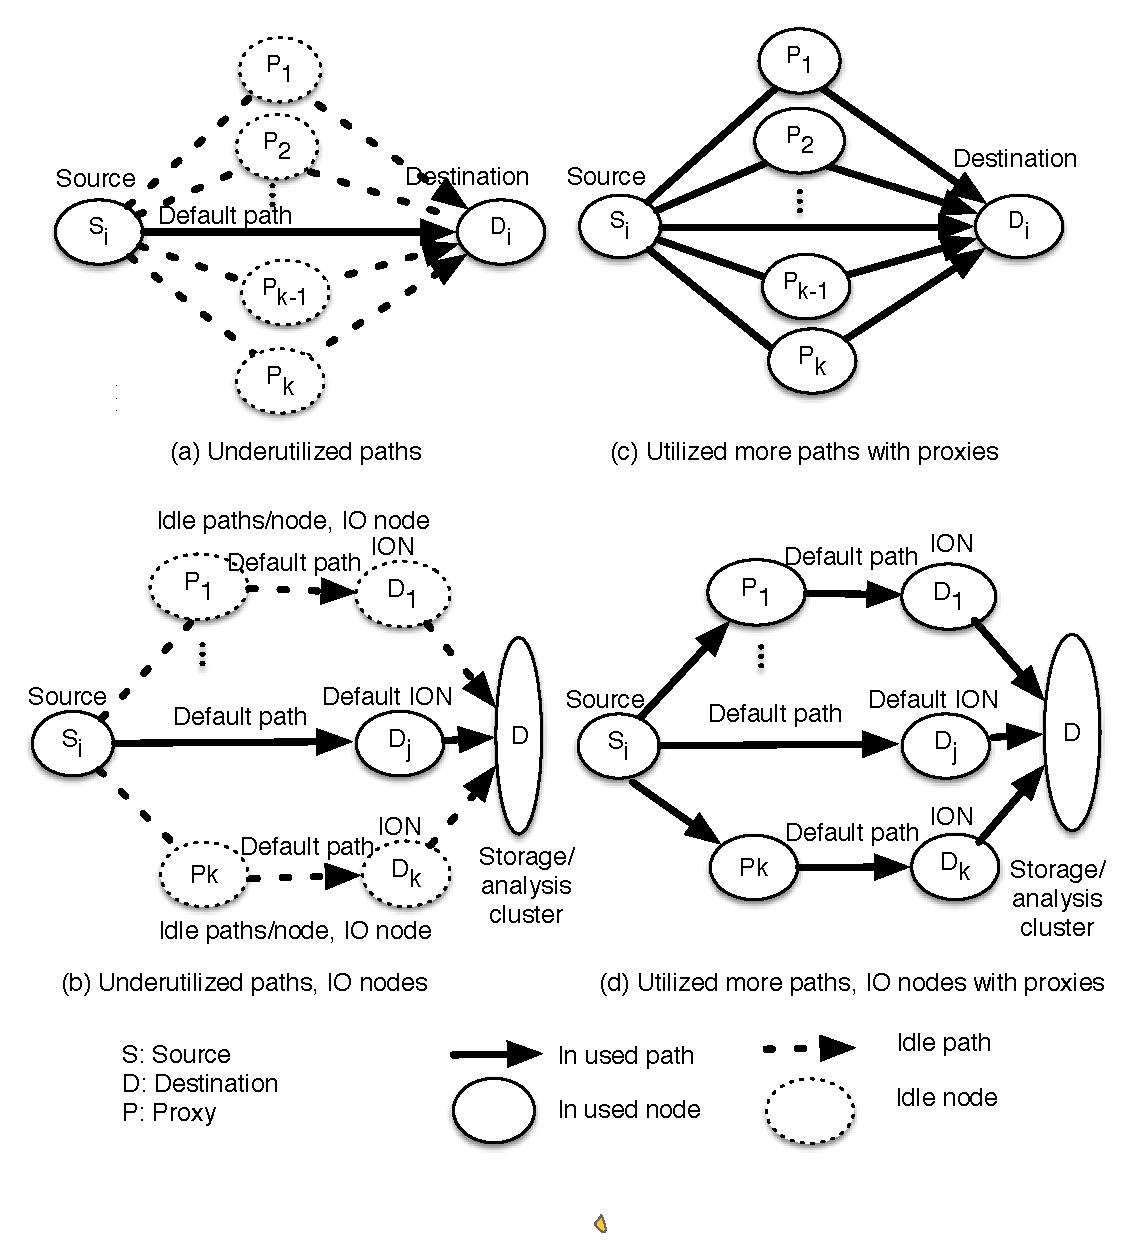
\includegraphics[scale=0.5]{multiply.pdf}
\vspace{-0.3in}
\caption{Data transfer with and without proxies}
\vspace{-0.1in}
\label{fig:multiply}
\end{figure}

To route data using multiple paths on a single-path-allowed system, we introduce intermediate nodes that are also compute nodes running the application and routing data at the same time. Following the default routing policy, we first route data from sources to the intermediate nodes and then from intermediate nodes to destinations. As shown in Figure \ref{fig:multiply}(c), by adding intermediate nodes, we make sure that we use as many I/O nodes as possible. Currently our routing function on the intermediate nodes causes overhead. We expect, however, that future systems will provide the functionality on nodes needed to achieve higher data movement throughput.  Knowing the routing policy, we should choose the locations of intermediate nodes to minimize the shared links and therefore maximize the throughput of data movement. Similarly, in Figure \ref{fig:multiply}(d), by adding the intermediate nodes, we can increase the number of I/O nodes and accordingly balance I/O workload. Clearly, using multiple paths in sparse data movement is critical for utilizing resources efficiently and subsequently for improving performance.

In the following sections, we describe our approach and associated techniques in detail.

\subsection{Multipath computation algorithms}
We model our data movement problem as a multipath computation problem when the interconnect network is given as a directed graph where vertices represent compute nodes and edges represent links connecting compute nodes. The bandwidth on each link is the capacity of the corresponding edge. On BG/Q where the compute nodes are allocated in a contiguous block, we can easily create a directed graph model for the allocated partition.

The model can have single or multiple sources and destinations. If more than one node is acting as source nodes and/or destination nodes, we create a {\em logical} source and/or a {\em logical} destination node and connect the logical node with real ones using {\em logical} links with infinite capacity. Our goal is to find disjoint paths that connect sources to destinations, yielding the highest possible throughput. To find such disjoint paths resulting in maximum flow, we use the Ford-Fulkerson algorithm \cite{ford1987maximal} extended with a breadth-first search (BFS). The algorithm has the runtime $\mathcal{O}(|V|^2*|E|)$, with $|V|$ being the number of vertices and $|E|$ being the number of edges. The runtime of the algorithm scales well with interconnect networks of supercomputers where $|E| >> |V|$.

In our work, we assume that the size of the data at the nodes that needs to be transferred out is approximately the same. Data has the same priority across all the nodes. The network is clean, so the capacity on each edge is entirely dedicated to our data movements.

Our implementation of the Ford-Fulkerson algorithm is as follows. We create a residual graph with full capacity and update it as we traverse the graph to find a path from a source node to a destination node. We use BFS to travel on the graph. We start at the source node and expand unvisited neighbors along each outgoing edge with positive capacities. The neighbors are then added to a queue and marked visited. As we travel, we record the previous node of each visited node. We continue the process until we reach the destination. As soon as we reach the destination, we traverse back to the source and update the residual graph. We continue the process until there is no path to go from source to destination with positive capacity.

Our modified Ford-Fulkerson algorithm produces the maximum flow together with paths that achieved that maximum flow. From the result,  we know at most how many paths a source may have. We assign paths to each source node in an incremental way, as described in Algorithm \ref{Alg:multipath}.

\begin{algorithm}
\caption{Multipath computation algorithm}
\begin{algorithmic}
	\STATE Use Ford-Fulkerson to find total number of disjoint paths P.
	\FOR {int i = 0; i $<$ P; i++}
	\FOR {each s in set of sources S}
	\STATE Find a path to one of its destinations, using BFS.
	\STATE When reaching its destination, go back and update the residual graph.
	\STATE Save the path for later transfers.
	\ENDFOR
	\ENDFOR
\end{algorithmic}
\label{Alg:multipath}
\end{algorithm}

In this algorithm, we iterate through the set of source nodes. For each source node, we find a path from source to destination and update the residual graph. We repeat the process until we run out of paths. In this way, paths are given in the increasing order of paths to the sources iteratively. By doing so, both short paths and long paths are distributed among the sources. Some sources may have more paths or have longer paths. Balancing between sources will be considered in future work. In a dense data movement pattern, there is usually one path for a source, but for a sparse data movement, multiple paths can be found. For symmetric data movement where all nodes move data in the same way, we can always find the maximum number of paths. However, if the data movement paths at source nodes are not the same, it may not return the maximum number of paths, resulting in less than maximum flow, but multiple paths can still be found.

The modified Ford-Fulkerson algorithm produces the maximum flow between two groups of nodes, as well as arbitrary paths resulting in maximum flow. However, these paths do not conform with default routing policies implemented in supercomputers. Therefore, to use the paths, we need to adjust the flow at every vertex on the paths; that is, we need to send data from one vertex to another one, make a copy, and send it to the next vertex on the paths. This implementation slows the data movement rather than speeding it. With a certain number of proxies introduced the performance gained is lower than the single-path data movement performance. Therefore, the number of paths as well as number of proxies is important in multiple-paths data movement.
%Next we present our approach of leveraging default routings to reduce the number of proxies.

\subsection{Leveraging routing policies to reduce number of proxies}
To route data between nodes in BG/Q, we use a default routing policy. On multiple paths we found that if the data movement between any two nodes on the path conforms with the default routing policies, we can remove nodes between the two nodes. By doing so, we can  still guarantee that data is moved along the desired path while reducing the number of proxies introduced, therefore increasing the performance. Our goal is to find as many subpaths as possible that conform with the default routing paths, thereby minimizing the number of proxies. To this end, we introduce routing rules into the maximum flow algorithm that we use.

In our algorithm, to go from a source node to a destination node, we explore unvisited neighbors and add them to a queue. As we explore and add next vertices in arbitrary order, the paths produced are also arbitrary. To make them conform with default routing policies, we use the routing policies to control the order in which we add the neighbors into the queue. Besides the constraint of routing, we also have another constraint for the number of proxies used along a path. As the number of proxies increases to certain number the discovering path degrades the performance, therefore being no longer useful. We need to discard the path to find a new one. In the following, we explain how to leverage routing policies on BG/Q.

In the Blue Gene/Q system, data is routed by the longest-dimension first and the shortest-dimension last policy. As soon as a message moves out from a source node, it routes along the highest dimension; it may need to change dimensions five times at most. For a message routing along a desired path, whenever the message routes from a higher to lower dimension, we do not need a proxy. But if we route a message from lower to higher dimension, we would need a proxy. We introduce the routing constraint and number-of-proxies constraint of BG/Q into breadth-first search as follows:

\begin{itemize}
\item The order of edges to add into the queue of BFS is reverse-of-routing orders. This is to make sure that the lowest-priority dimension can be discovered first. The lowest-dimension-first path would need more proxies; being able to select the next nodes first would reduce the number of proxies along the path. By doing so, we can balance the number of proxies among multiple paths.
\item If it is possible, do not use proxies. Whenever we need to add an edge that data moving by that edge has higher priority that the previous edge, we need to add a proxy.
\item Constraint on total number of proxies: if the number of proxies used is more than the constraints, no longer explore that direction.
\end{itemize}

\subsection{Pipeline technique for data movement}
Since we have to transfer data from the source node to the proxies first, and then from the proxies to the destination, we need to store data at a proxy. If we store the entire message at the proxy, it takes time to wait until the entire message arrives and  then start injecting the message into the network to the next proxy. To reduce the time to wait, we split the message into smaller messages and transfer the messages using a pipeline such that storing messages and sending messages at a proxy can run concurrently.

For each proxy, requests to wait for data are posted at the beginning. After that, the proxy needs to iterate through the list of requests while checking whether data is ready to forward. To implement the pipeline, we create two threads at each proxy: one thread for receiving data and the other for forwarding data. A message is split into smaller messages with a certain size called the window size. The size of the window depends on the message size and is determined based on experiments. Within each message we embed the information of how data will be processed at the next node such as destination, address of the message in the destination's buffer, and the path Id that the next node should use to forward the message. The pipeline technique can be used in any system and yields significant improvement as we show in Section \ref{sec:microbenchmark}. With small messages, however, we still suffer performance degradation. The reason is that the control overhead in small messages is significantly large compared with the message size itself. Using low-level communication libraries can help reduce the control overheads. On BG/Q, PAMI is a low-level library for communication that improves the transfer of small messages. In the next subsection, we present our work of using PAMI on BG/Q to improve data movement throughput.

\subsection{Improving data movement performance using PAMI}
PAMI supports both one-sided and two-sided communication. It supports both small immediate communication and rendezvous large-message communication. In our study, we use one-sided communication for messages transfer and immediate send for control data. In sending and receiving data events, PAMI supports a callback function to let a sender and receiver know whether the event of sending/receiving has been done at either side.

\begin{figure}[!htb]
\centering
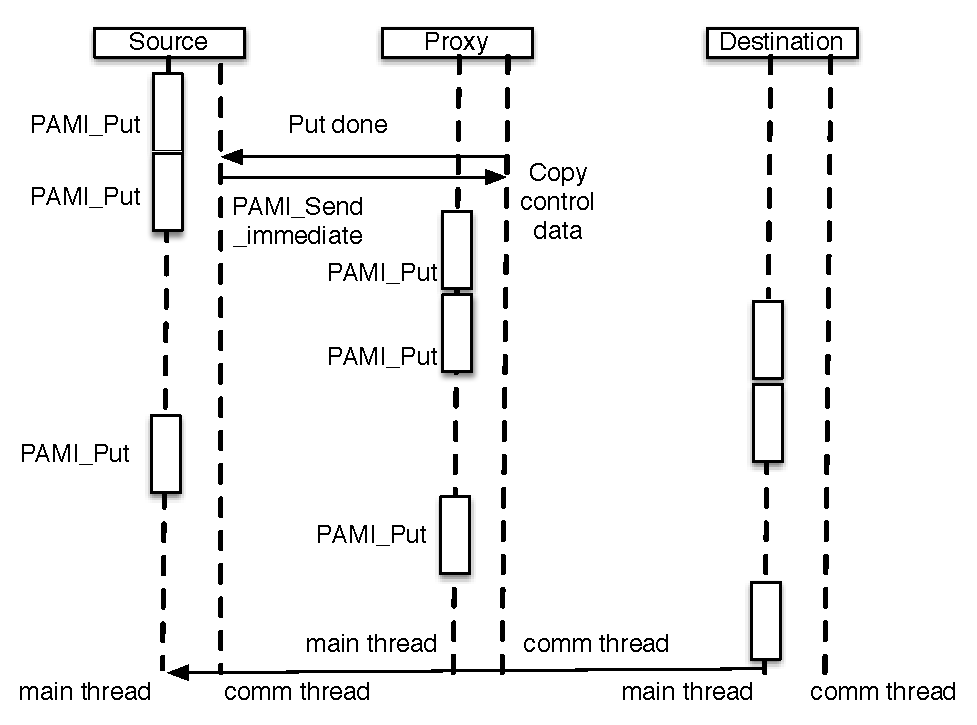
\includegraphics[scale=0.5]{pami_pipeline.pdf}
\caption{Using pipelining technique with PAMI to eliminate the waiting time at proxy and reduce control overheads}
\label{fig:pami_pipeline}
\end{figure}

As depicted in \ref{fig:pami_pipeline}, in the main thread of the source, we keep transferring data to windows of its proxies using \textit{PAMI\_Put}. Its comm thread running on the background is notified whenever the data is completely put on a proxy's side. The comm thread then uses \textit{PAMI\_Send\_immediate} to let the proxy know that the data is ready. It also sends the control data of where and how to process the data with the \textit{PAMI\_Send\_immediate}. Each proxy needs to set up a callback function to process the control data sent to it. The callback function copies control data to a queue and informs the main thread. The main thread at each proxy plays the same role as the main thread of the source node. The size of the window for each message size is also determined empirically.

In the next section, we present the efficacy of our solution on Mira through a set of microbenchmarks.

\section{Microbenchmarks}
\label{sec:microbenchmark}
In this section, we elucidate the efficacy of our approaches using a set of microbenchmarks.
%As mentioned in the previous section,
We introduce proxy nodes to implement multiple paths for data movement in the user space. By doing so, we introduce extra processing time at the proxies to receive, buffer, and forward the data. We can mitigate the effect of this at the proxies by using a pipelining mechanism to overlap these stages; and we further improve the performance by overcoming the overhead in MPI's data movement by leveraging PAMI, the lower-level BG/Q messaging layer.
%GWP - do you really still need to state that PAMI is low-level 
In the following subsections we show that we can achieve close to peak achievable bandwidth when transferring data between two nodes, with data being forwarded by using an intermediate node. For most of the experiments below, we used MPI\_Put/PAMI\_Put (one-sided communication) to transfer data with 1 MPI/PAMI rank per node. For each data transfer we vary the data size in powers of 2. Each experiment was repeated 20 times, and the average of the results are reported. We start with benchmarks showing the efficacy of pipeline technique using MPI.

\subsection{Efficacy of proxies and pipeline technique}

In this microbenchmark we transfer data between two nodes through an intermediate nodes using pipelining, and we compare results with transferring data without using the pipeline and with a direct transfer (default) scheme. We varied the data size from 1K  to 128 MB.

\begin{figure}[!htb]
\centering
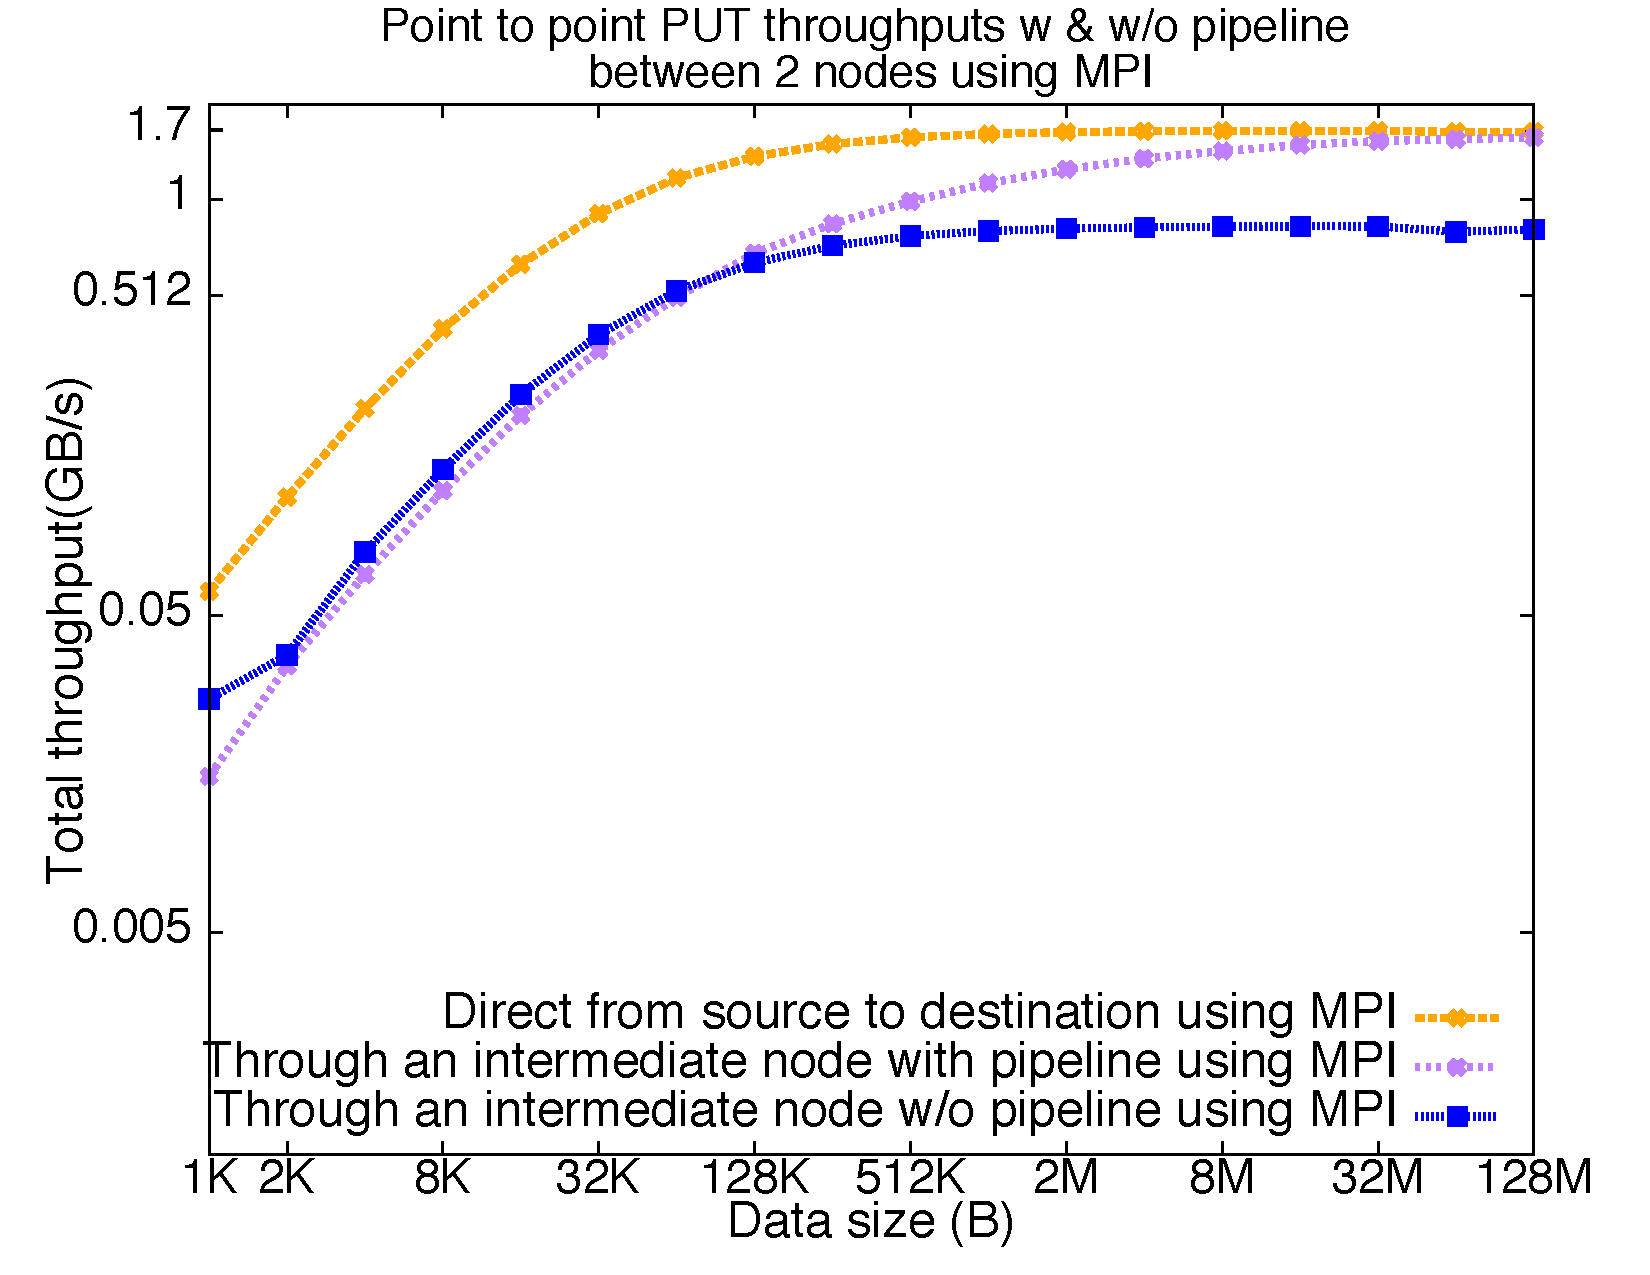
\includegraphics[scale=0.3]{pipeline_mpi.pdf}
\caption{Using pipelining technique to mitigate the waiting time at proxy nodes}
\label{fig:pipeline_mpi}
\end{figure}

Figure \ref{fig:pipeline_mpi} shows that transferring data through a proxy without using pipelining results in a 50\% hit in performance over a direct transfer. The reason is that the proxy needs to wait until all the data is ready before forwarding it to the destination. By using pipelining, for a message less than 64 KB,  pipelining does not improve performance; however, for a message size larger than 64 KB, pipelining demonstrates an improved performance. At a  message size of 1 MB, 2 MB, and 4 MB, we achieve 70\%, 80\%, and  90\%, respectively, of the direct transfer bandwidth; and with larger messages, we achieved a similar performance. Thus, with large messages, the pipelining technique can be used to transfer data through proxies. With small messages, however, the performance gained is insignificant. Much of the performance overhead is due to the underlying rendezvous protocol design in MPI on BG/Q. 
%ext, we use PAMI to improve the performance for small messages.
In the next subsection, we show the efficacy of using PAMI on transferring small messages.

\subsection{Efficacy of PAMI on multiple paths data movement}
In this subsection, we demonstrate that with the optimal window size for pipelining and PAMI we can gain near-maximum performance by direct transfer.

\begin{figure}[!htb]
\centering
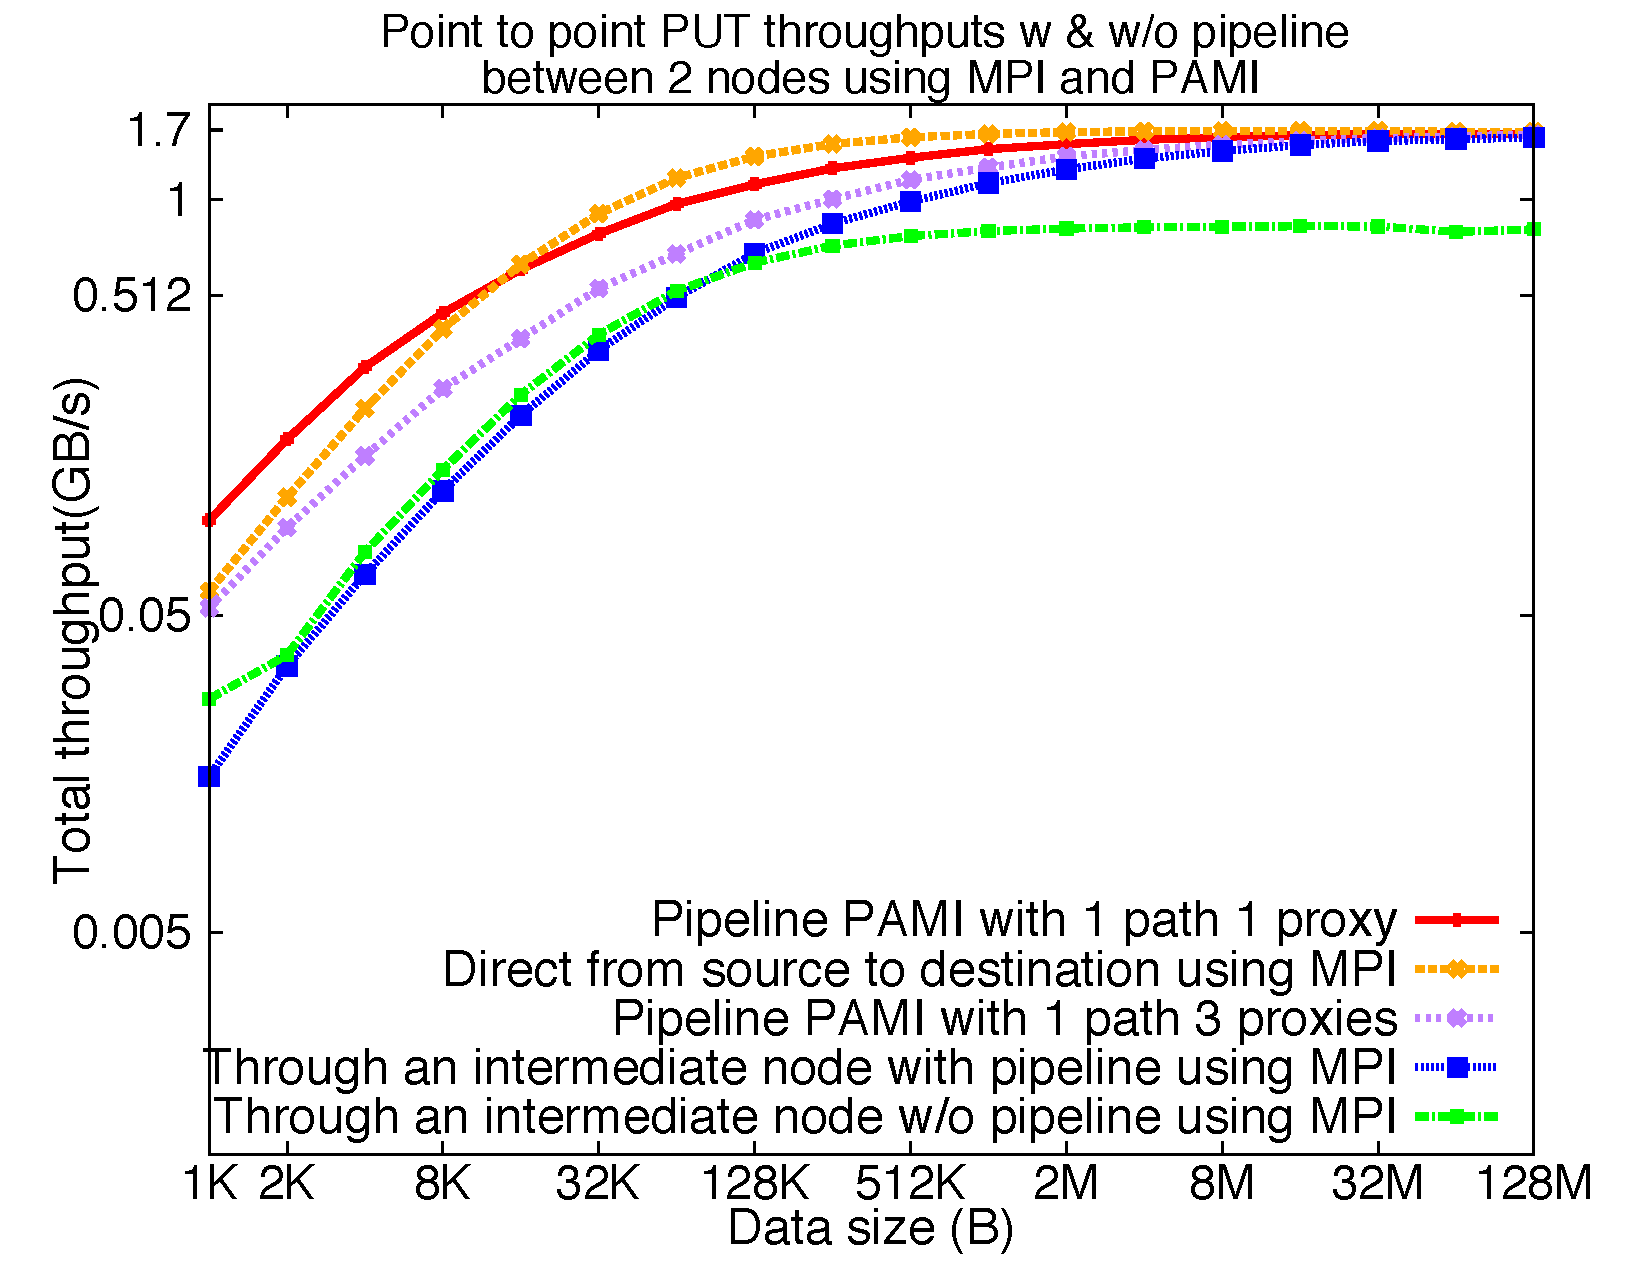
\includegraphics[scale=0.3]{pipeline_pami.pdf}
\caption{Using PAMI with pipeline technique to mitigate the waiting time at proxy and reduce overheads}
\label{fig:pipeline_pami}
\end{figure}

In this experiment, we transfer data from a source node to a destination node through a proxy with pipelining  and use PAMI with 1 proxy compared with the previous approach using MPI. We use PAMI\_Put to transfer data and PAMI\_Send\_immediate to transfer control information. We vary the data size from 1 KB to 128 MB. The results are shown in Fig. \ref{fig:pipeline_pami}.

As the figure shows, for message sizes less than 16 KB, using PAMI and pipeline results in a better throughput than does direct transfer using MPI. The reason is that PAMI has less control overhead than does MPI. With messages having sizes from 32 KB to 2 MB, our solution's throughput is close to direct transfer using MPI. With messages larger than 2 MB, the performance is similar to that with MPI and achieves the maximum of ~1.7 GB/s that one can achieve using a single link/route on BG/Q. Thus, using pipelining together with PAMI is an attractive alternative for data movement using a proxy node.

So far, we have demonstrated that with a pipeline technique and PAMI we can gain near-maximum throughput for a single path. Next, we evaluate the efficacy of using multiple paths for data movement between a source and a destination. In this experiment, we use a partition of 512 nodes on BG/Q and transfer data between two nodes.  With this allocation (and larger ones) we start to see the benefit of a full torus on all dimensions where each node has 9 neighbors (10th link is on the same node). 

\begin{figure}[!htb]
\centering
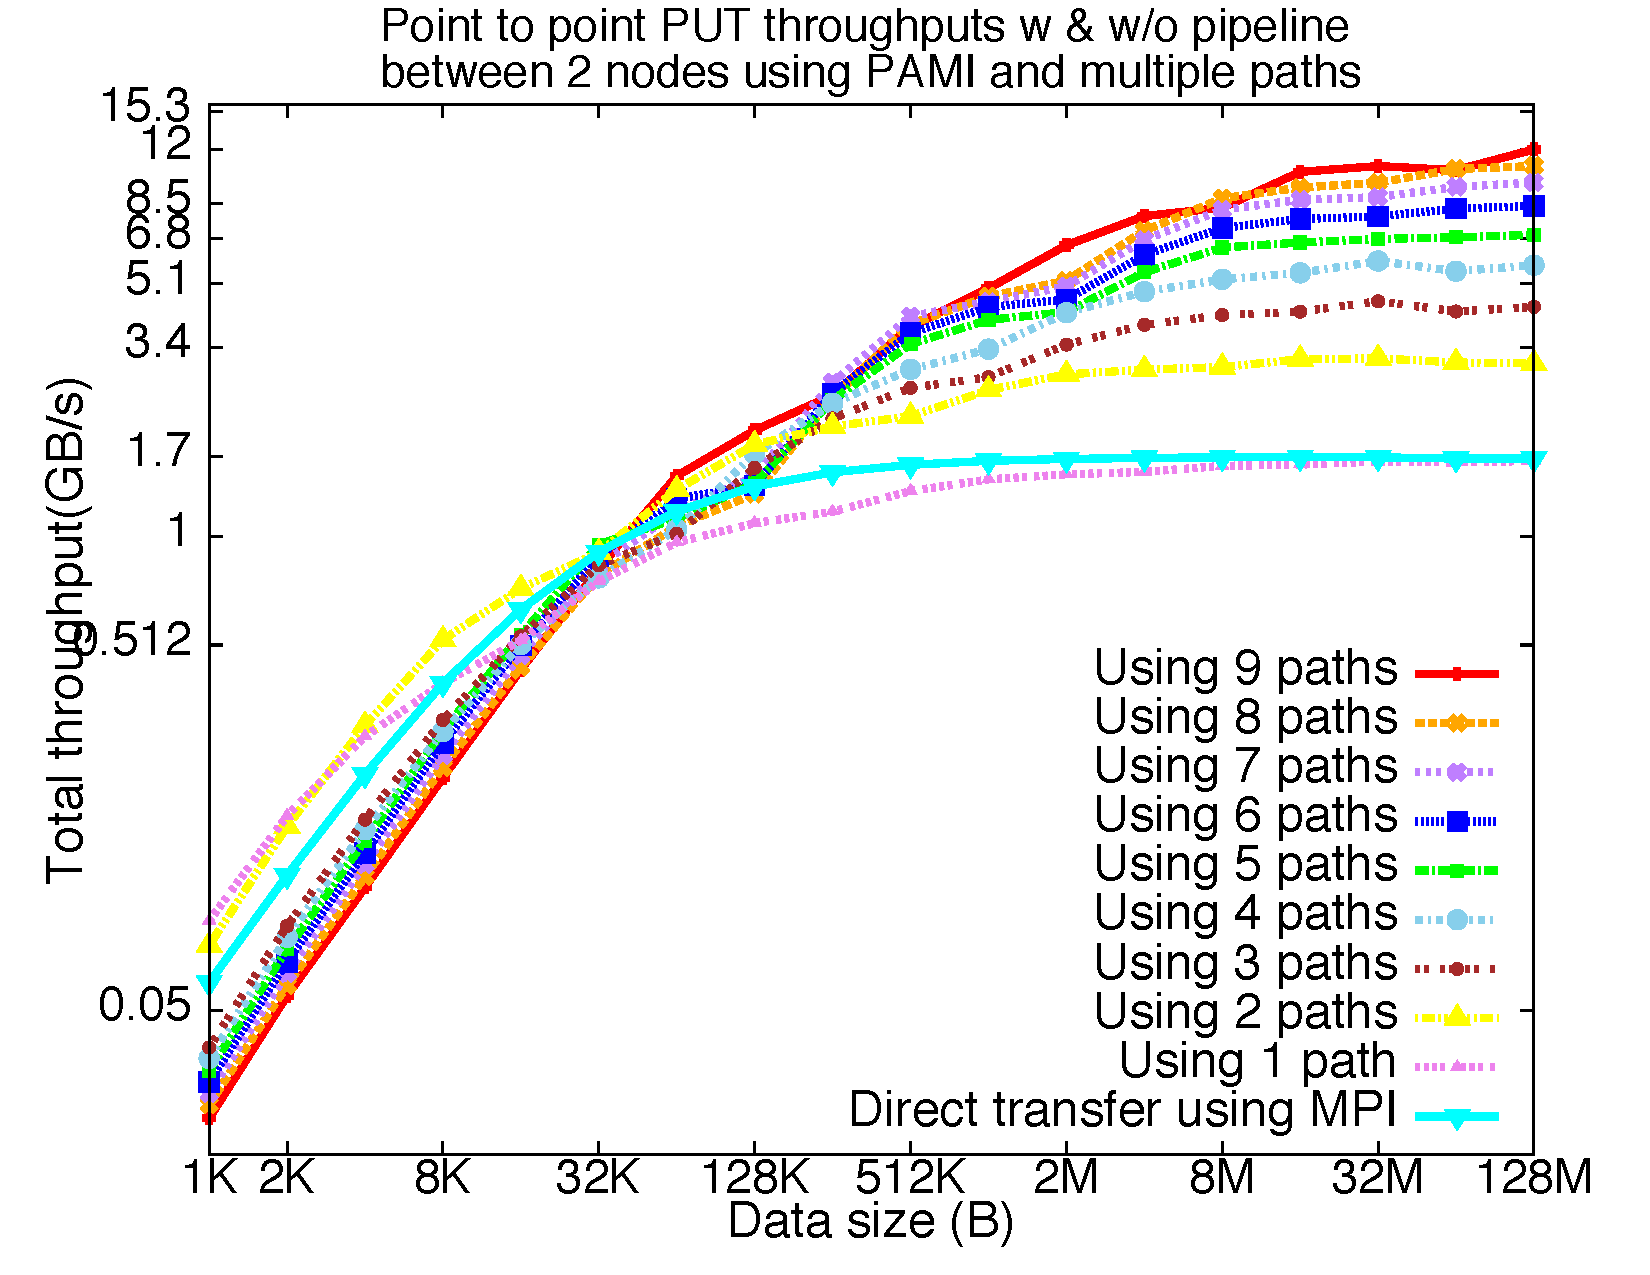
\includegraphics[scale=0.3]{pami_multipaths.pdf}
\caption{Using 9 paths to transfer data between two nodes}
\label{fig:pipeline_proxies}
\end{figure}

In our experiment, we increase the number of paths used for transferring data from one path to nine paths as we vary the message size from 1 KB to 128 MB split equally among all paths. As Fig. \ref{fig:pipeline_proxies} shows, by exploiting all 9 links to transfer data we achieve a throughput of 12 GB/s  or ~80\% of 15.3 GB/s max achievable throughput per transfer by exploiting all nine links. For messages larger than 32 KB, we increase the number of paths, the performance increases linearly from 2$\times$ to 7.8$\times$ over the default direct transfer used by MPI. We can also see that with small messages, using all nine paths actually degrades performance because of the control overhead. The number of paths should be chosen according to message size: that is, if the message size is less than 4 KB, we need a single path; between 4 KB and 16 KB we need two paths; between 16 KB and 32 KB we need three paths; and so on. Thus, depending on the message size, we should choose an appropriate number of paths to achieve the best performance.

The microbenchmarks show that using multiple paths for data movement with pipelining and PAMI can achieve significant improvement on BG/Q. To achieve the best performance (i.e., highest throughput), we need to dynamically choose several factors, including the optimal window size and the number of paths; and we need to adjust the size of data for each path since some paths are longer with more proxies than others. The microbenchmarks also show that the performance gained would suffer significantly when the number of proxies increases. In the next section, we show how our solution effectively leverages routing policies in order  to reduce the number of proxies needed and thereby increase total performance.

\subsection{Efficacy of leveraging routing policy on performance}
In this experiment, we use nine paths to transfer data from a source node to a destination node. The number of proxies in between the 2 nodes on different paths varies from one to four. By applying our algorithm for leveraging routing policies we can reduce the number of proxies on the longest paths to three. The performance results are shown in Fig. \ref{fig:pami_shorterpaths}.

\begin{figure}[!htb]
\centering
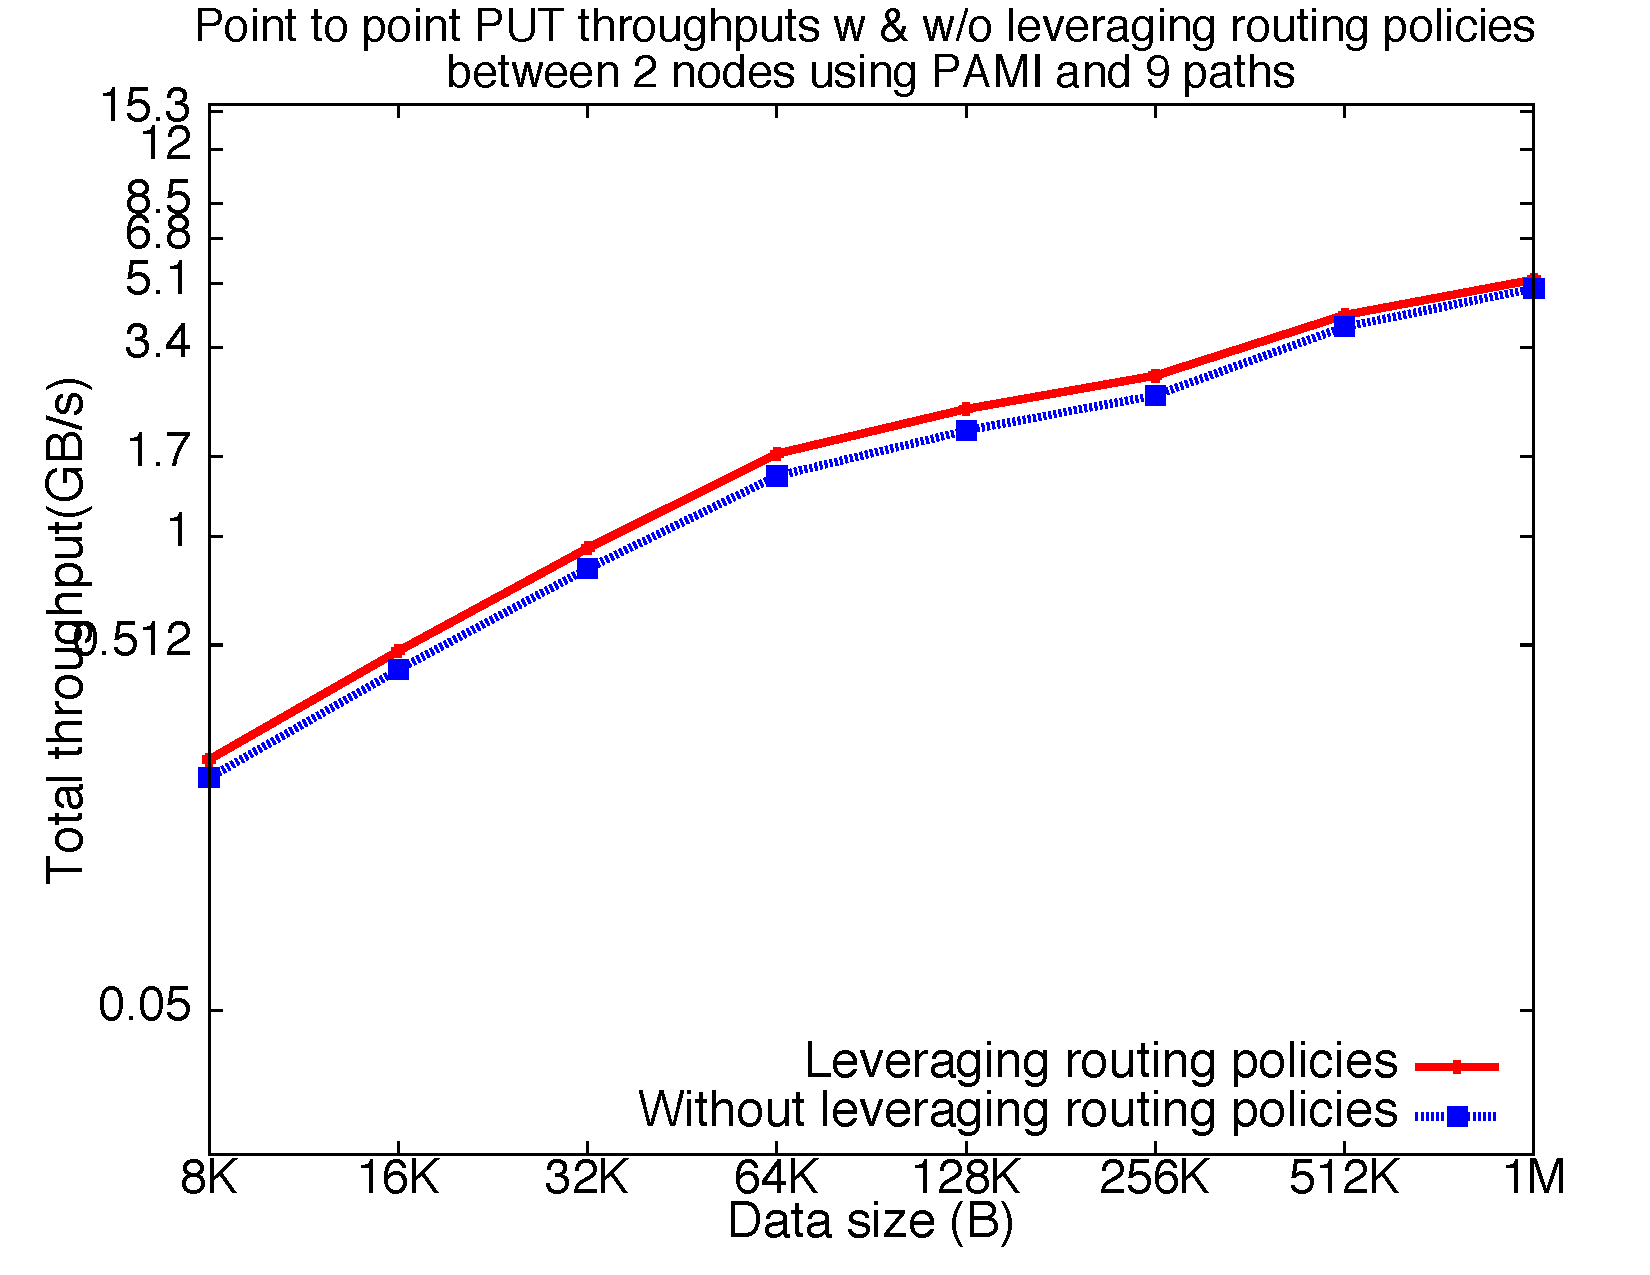
\includegraphics[scale=0.3]{pami_shorterpaths.pdf}
\caption{Leveraging of the routing policy to reduce number of proxies introduced}
\label{fig:pami_shorterpaths}
\end{figure}

The performance gained is modest, only $\sim$10\% for medium-sized messages. This is due to the small number of proxies removed in comparison with number of proxies remaining. For small messages, control overhead dominates and cancels the improvement. With large messages, the time to transfer the actual data makes the improvement negligible. In certain cases where longer paths exist, however, we believe that performance gains can be improved further with this scheme. 


\subsection{Optimization of window size}

To use pipeline efficiently, we need to determine optimal size of transfer window for pipelining for each message size; A single message is split into a number of transfers.  Figure \ref{fig:pipeline_winsize} depicts the effect of transfer sizes on data movement. In this experiment, we vary the message size from 16 KB to 32 MB and the transfer size from 512 bytes up to 2 MB or the message size if the message size is less than 2 MB.
%GWP - not sure about the "or the message size..." - what does it go with in the sentence?
We increase the transfer size and message size twice after each step. We transfer the data using PAMI\_Put from the source node to a proxy node and then to a destination node in a partition of 32 nodes, using only one process per node. These nodes were 2 hops away from each other, but a different selection of nodes would produce the same results. The results are shown in Fig. \ref{fig:pipeline_winsize}

\begin{figure}[!htb]
\centering
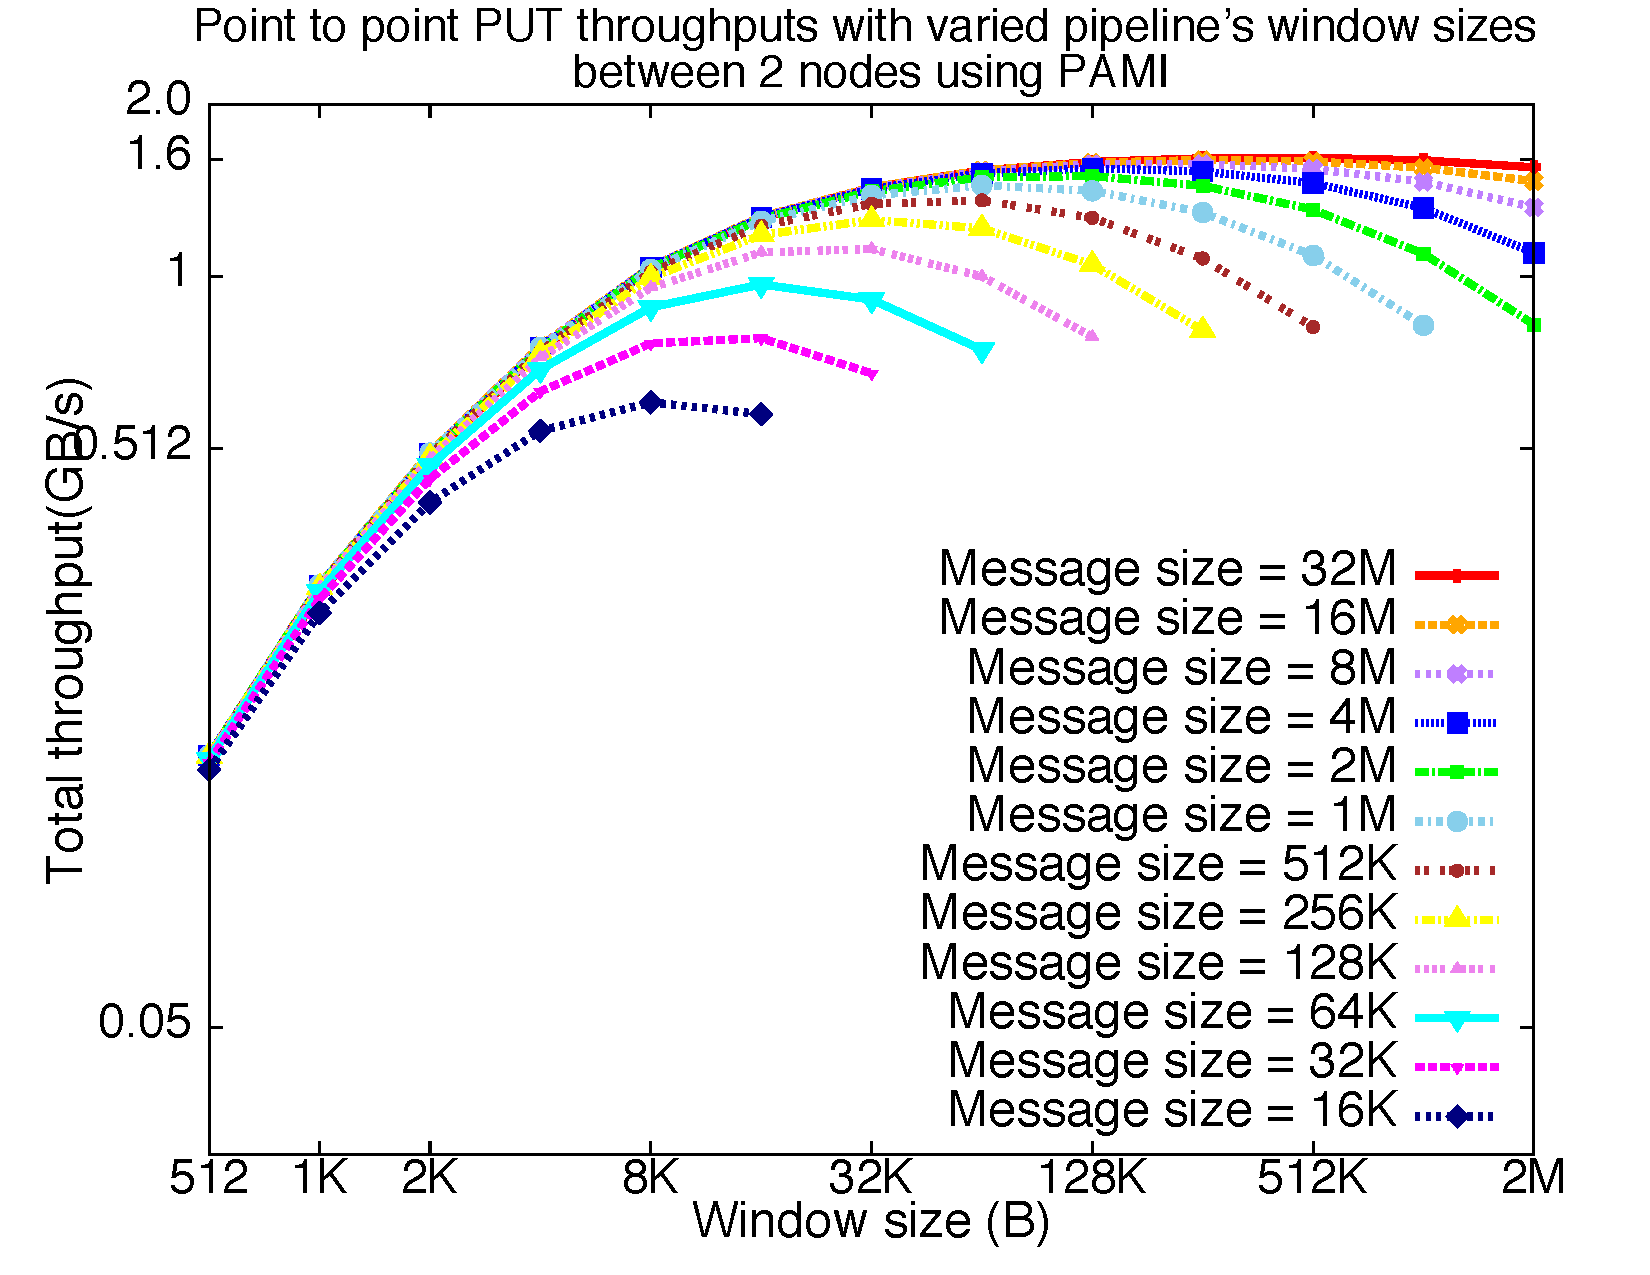
\includegraphics[scale=0.3]{winsize_pami.pdf}
\caption{Window size and performance when using PAMI}
\label{fig:pipeline_winsize}
\end{figure}

We can see that for messages with size less than 16 KB, direct transfer results in better throughput. The reason is that control overhead is higher when transferring a few small messages instead of transferring a single message. With messages with size 16 KB or larger, the pipeline technique results in better performance with an optimal transfer size. Depending on message size the optimal size varies; that is, to transfer a 2 MB message, a transfer size of 128 KB results in the best throughput. From the figure we also see that if we choose a nonoptimal transfer size, the performance drops significantly. Thus, the transfer size for pipelining is critical in order to achieve the highest bandwidth in multipath data movement.

\subsection{Efficacy of multipath data movement between two groups of nodes}
In this subsection, we show the efficacy of our solution in moving data between two groups of nodes in Mira. This is typically the case for coupling the data between multiple physics modules.

In BG/Q compute nodes are allocated as a contiguous block. In this experiment, we transfer data from a contiguous block of 64 nodes to another contiguous block of 64 nodes in a 512-node partition using multiple paths and a single path with MPI\_Put. We use one process per node, and each node from the source block transfers a message to its corresponding node in destination block in a symmetric way. We vary the message size from 1 KB up to 128 MB. The results are shown on Fig. \ref{fig:mncoupling_mira}

\begin{figure}[!htb]
\centering
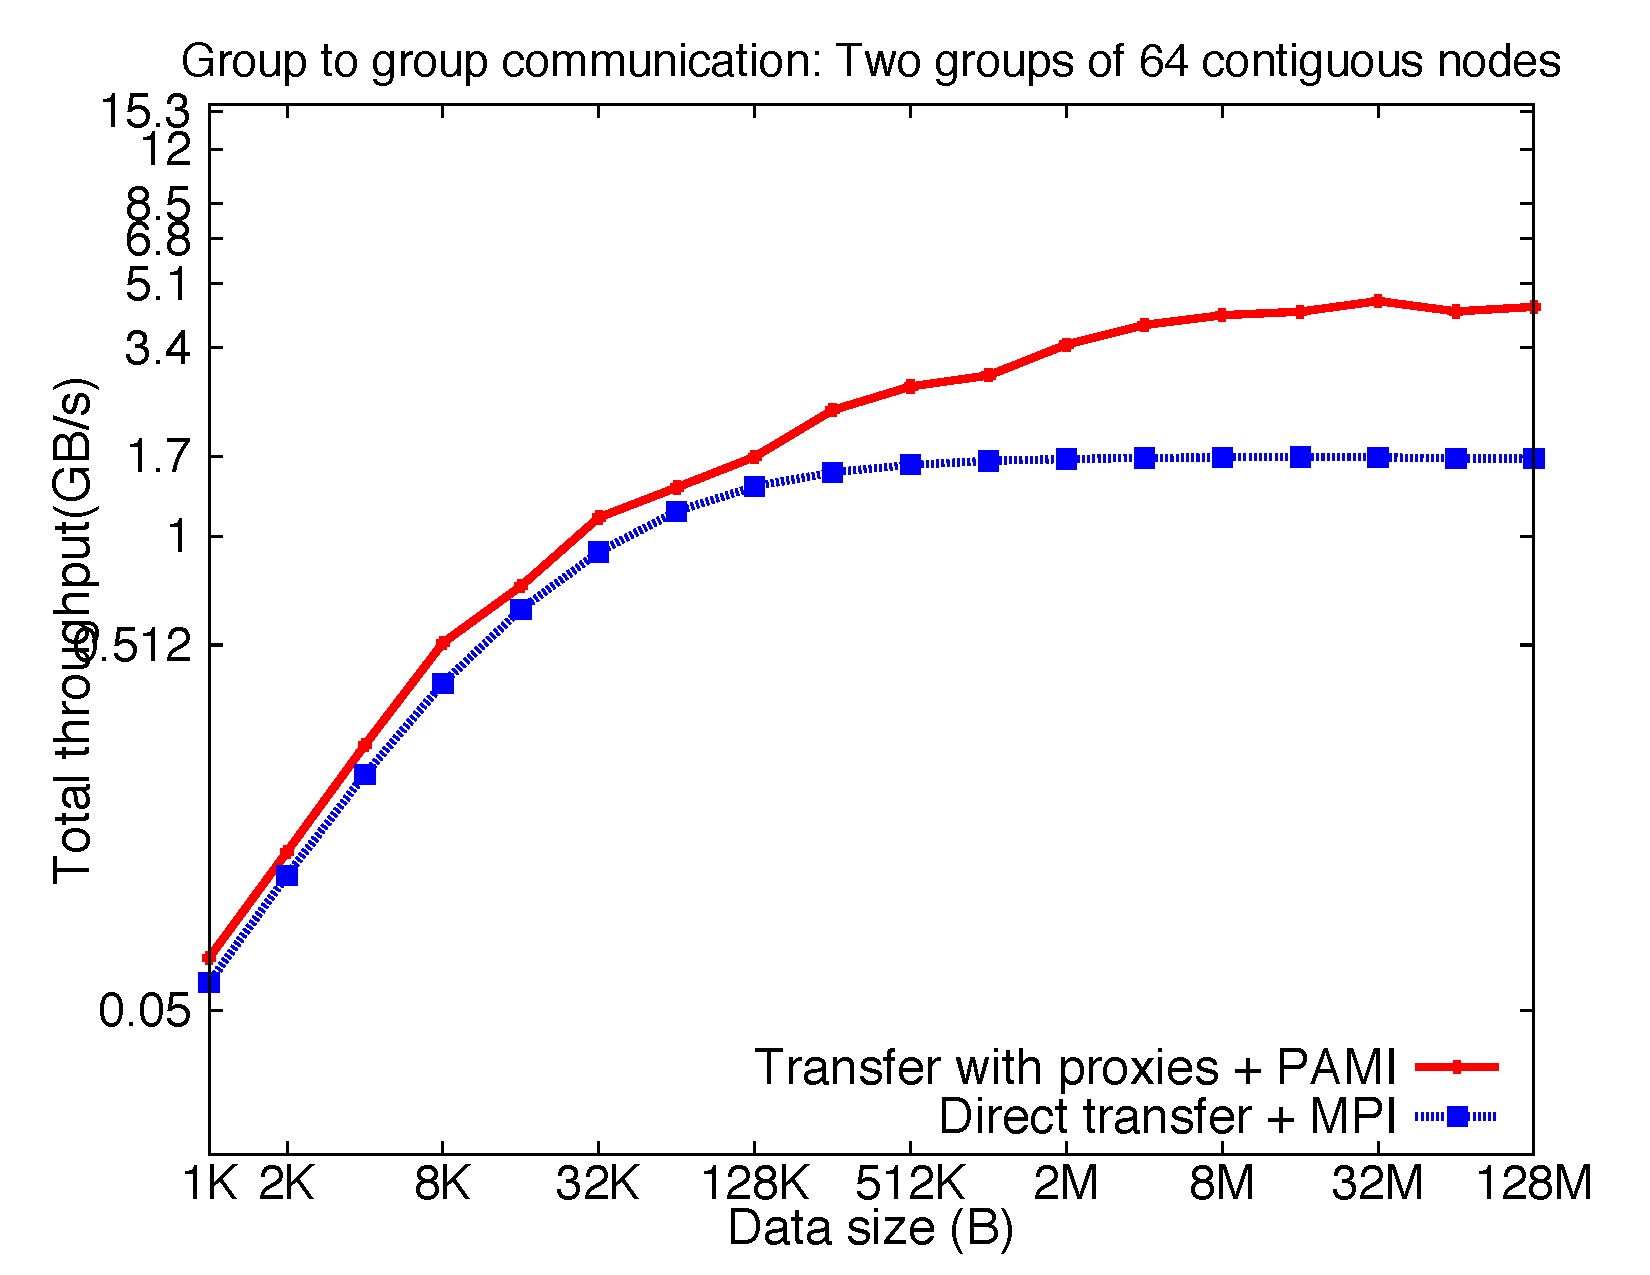
\includegraphics[scale=0.3]{mncoupling_mira.pdf}
\caption{Data movement throughput between two groups of 64 nodes each in a 512-node partition on Mira}
\label{fig:mncoupling_mira}
\end{figure}

With the data movement requirement, the Ford-Fulkerson algorithm returned maximum flow with at most three paths per node. As the figure shows, with a message size more than 2 MB we can achieve ~4.7 GB/s or almost 3$\times$ better than single-path data movement. This result shows that our solution can work well for data movement between two blocks of nodes when the data movement paths are symmetric.

\section{Synthetic and application I/O benchmarks}
\label{sec:appbenchmark}
In this section, we demonstrate the efficacy of our approaches using a set of synthetic benchmarks and application-level benchmarks.

\subsection{Synthetic benchmarks}
We perform a weak-scaling study with two sparse data patterns, and we scale the number of cores from 2,048 to 131,072 cores on the Mira BG/Q system. We use a synthetic I/O benchmark wherein the I/O distribution has the following patterns:

\begin{itemize}
\item Pattern 1: Uniform distribution of data, where the data size of an MPI rank is uniformly distributed between 0 and 8 MB.  Data is generated by using the \textit{srand()} and \textit{rand()} functions in C/C++ and using the \textit{time(NULL)} as a seed.  The total data size is about 50\% of the dense data size. The distribution of the data is shown in Fig. \ref{fig:uniform}
\item Pattern 2: Pareto distribution of data, where most of the MPI ranks have a data size of 0 bytes or very small size, and a few of MPI ranks have a data size of approximately 8 MB. The total data size written out is about 20\% of the dense pattern size. The distribution of the data is shown in Fig. \ref{fig:pareto}
\end{itemize}

Pattern 1
%data sizes are uniformly distributed among nodes.
is typical of applying an analysis to the entire dataset; depending on the result of the analysis, we might have sparse patterns across the entire volume.

\begin{figure}[!htb]
\vspace{-0.2in}
\centering
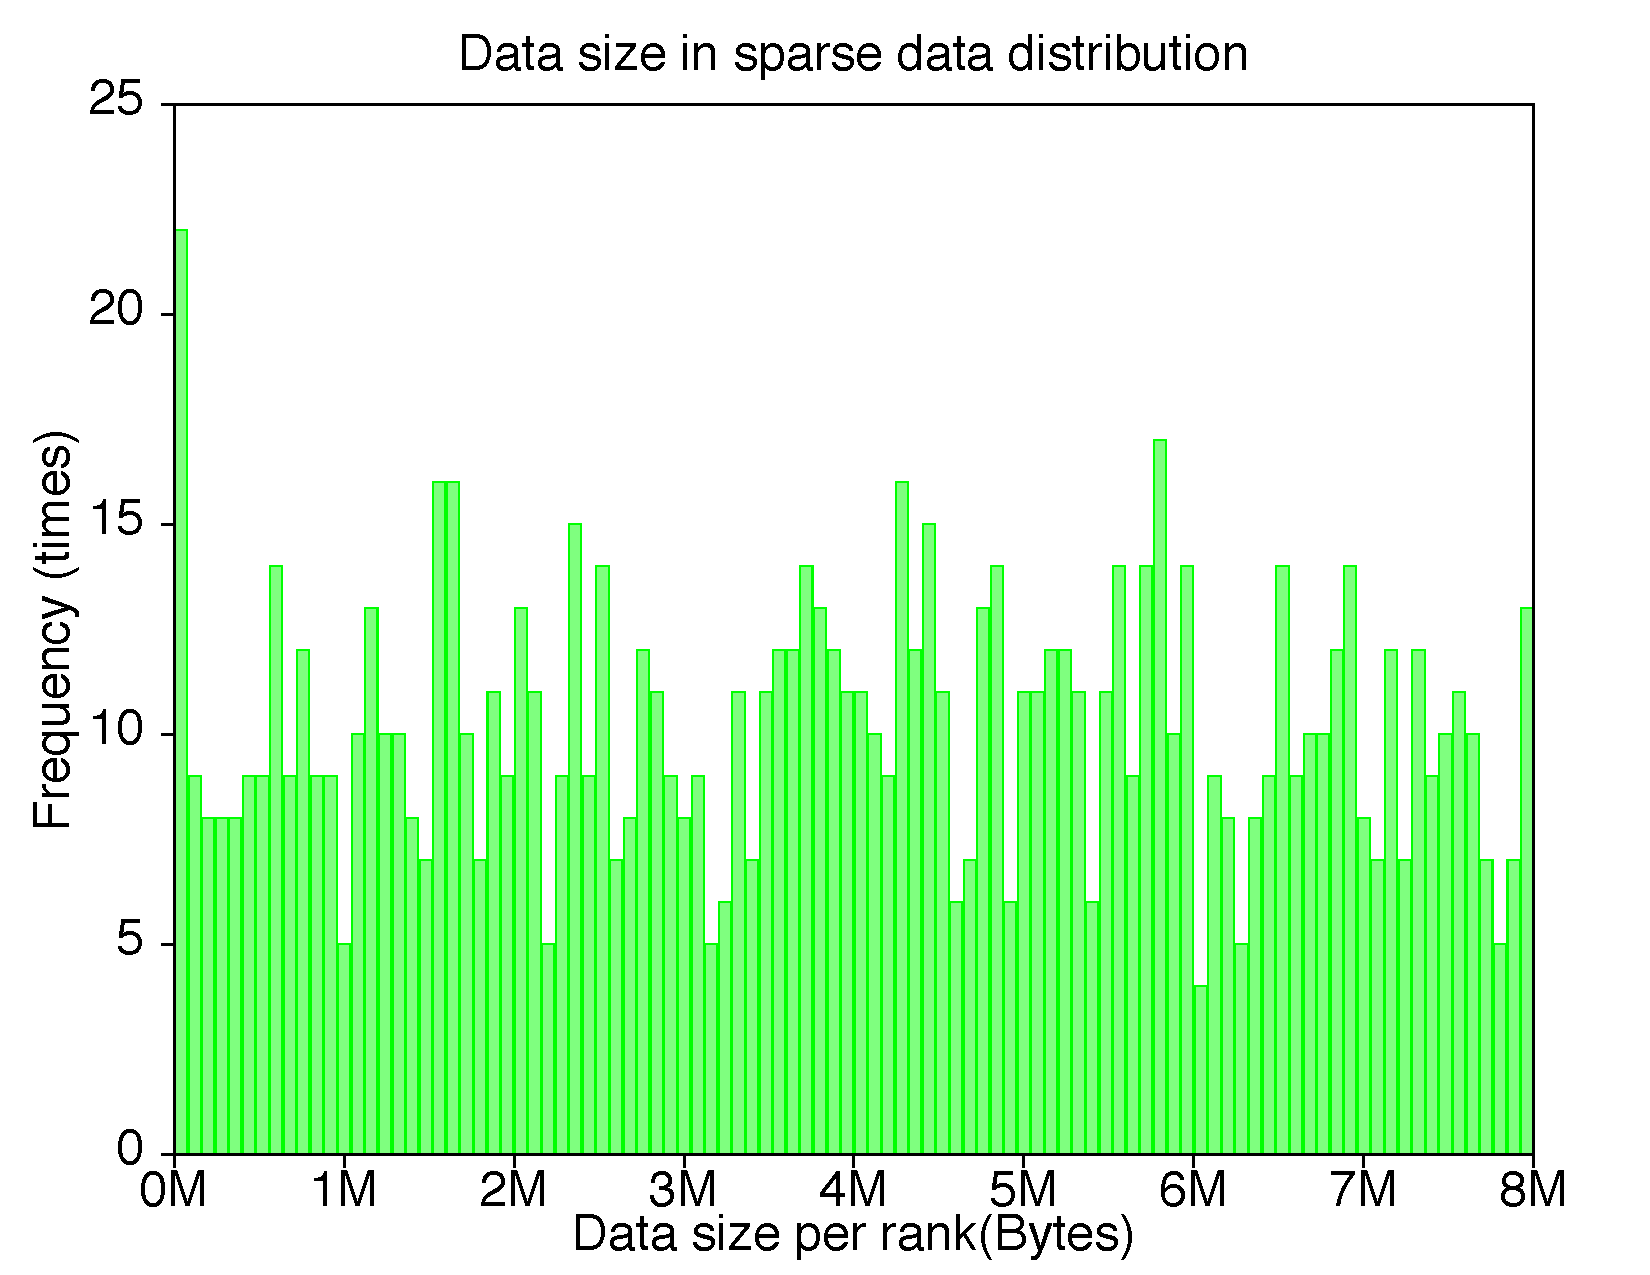
\includegraphics[scale=0.3]{uniform.pdf}
\caption{Pattern 1: Histogram of data sizes for 1,024 processes using the time(NULL) function with size from 0 to 8 MB}
\label{fig:uniform}
\vspace{-0.1in}
\end{figure}

Pattern 2, on the other hand, represents an in situ analysis applied to a region of interest, such as a  region of turbulence, that spans a small subset of MPI ranks and needs to be written out to storage.

\begin{figure}[!htb]
\vspace{-0.1in}
\centering
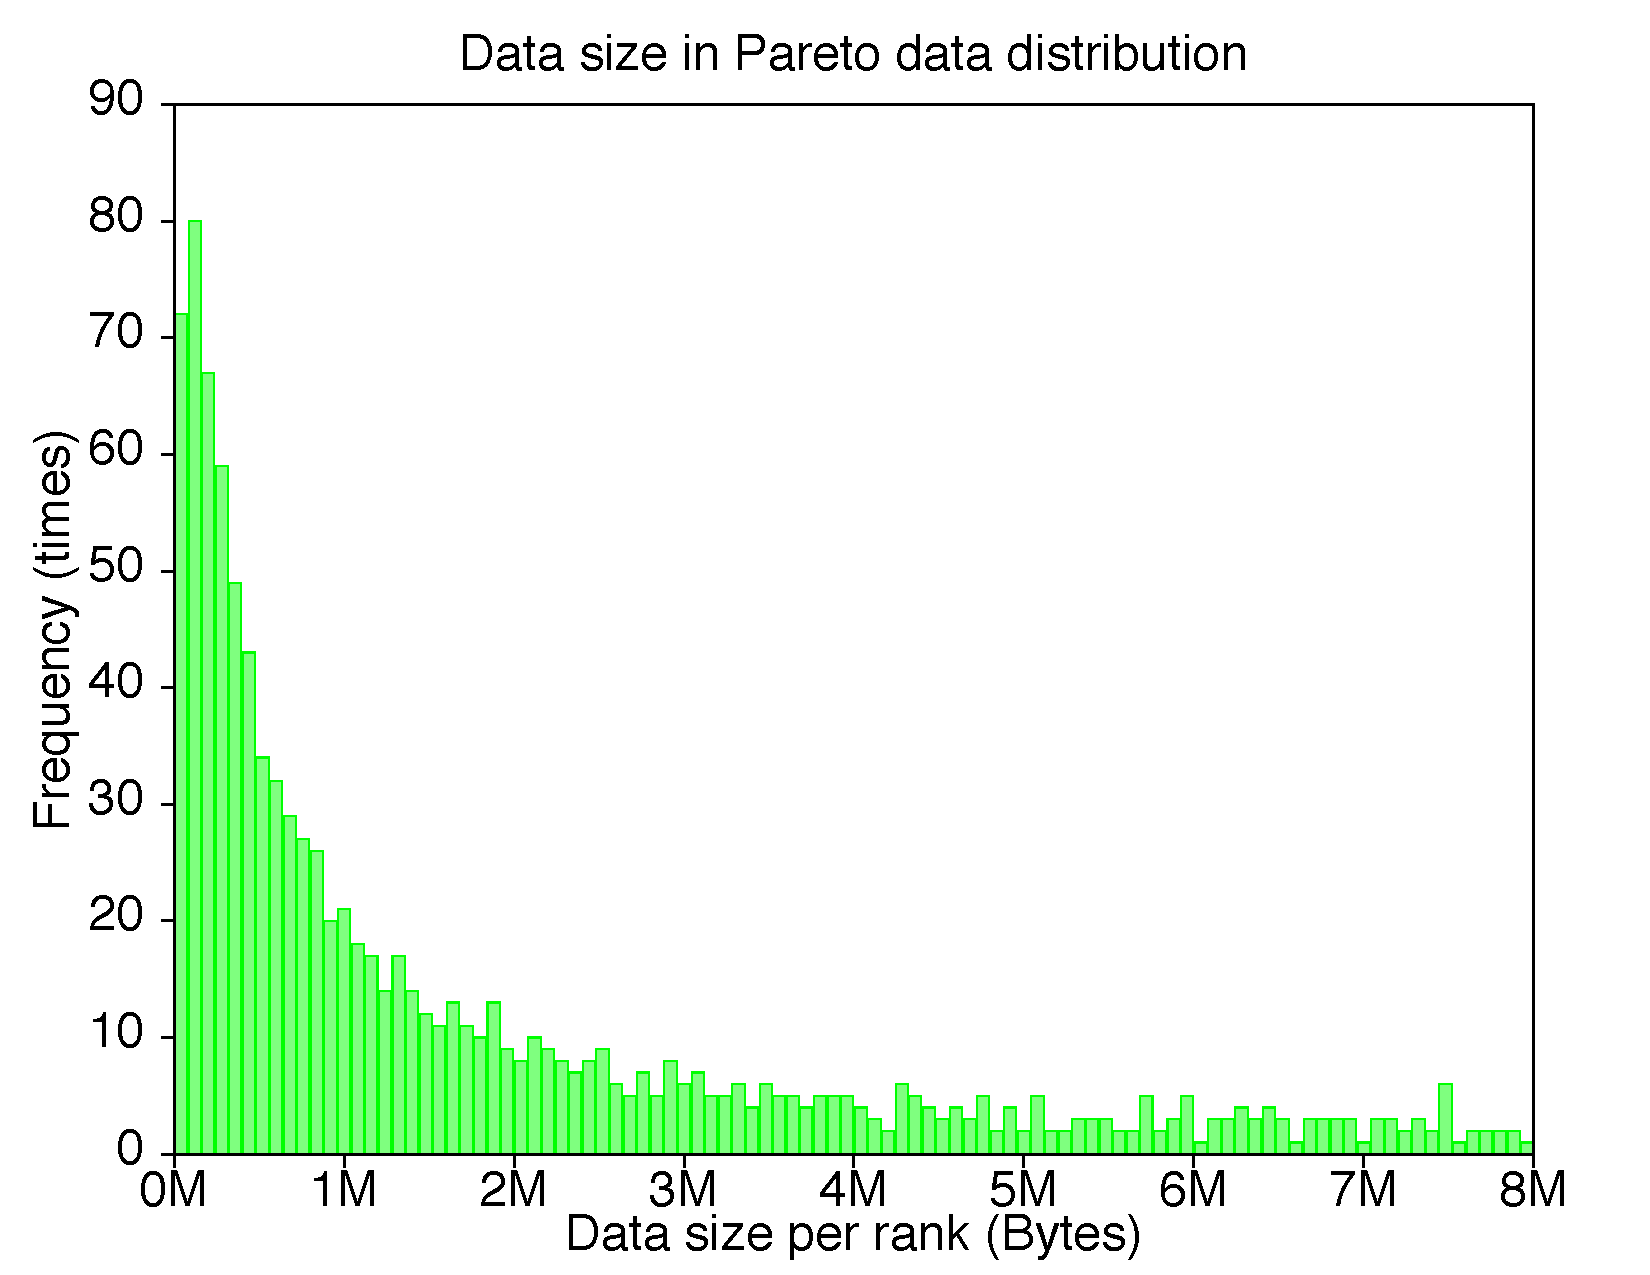
\includegraphics[scale=0.3]{pareto.pdf}
\vspace{-0.1in}
\caption{Pattern 2: Histogram of data sizes of 1,024 processes using Pareto distribution function with size from 0 B to 8 MB}
\label{fig:pareto}
\vspace{-0.1in}
\end{figure}

%\subsection{Efficacy of using multiple paths to move data between compute nodes and I/O nodes}

On BG/Q, I/O data is routed from the compute nodes to the I/O nodes through a set of special compute nodes called bridge nodes. In this benchmark, we use our multipath data movement heuristic to transfer data along multiple paths from the compute nodes to the bridge nodes and then write this data out. We perform two experiments. First, we write the data to /dev/null on the I/O nodes so as to mitigate the effects of the storage systems and understand the efficacy of our data movement algorithm. Next, we write the data out to the GPFS parallel file system to get the overall end-to-end I/O performance. In the benchmark, we use the two sparse data patterns. For Pattern 1, we select 10\% of the nodes to write data out, while the other nodes do not write out any data. For Pattern 2, every node has data, but the data size varies: some nodes have a lot more data than other. On Pattern 1, we write roughly 8 GB at 2,048 cores and 274 GB of data at 131,072 cores. On Pattern 2, we write ~3.4 GB at 2,048 cores and 119 GB of data at 131,072 cores. We compare the performance of performing I/O for the two data patterns using our approach and default MPI collective I/O.

\begin{figure}[!htb]
\centering
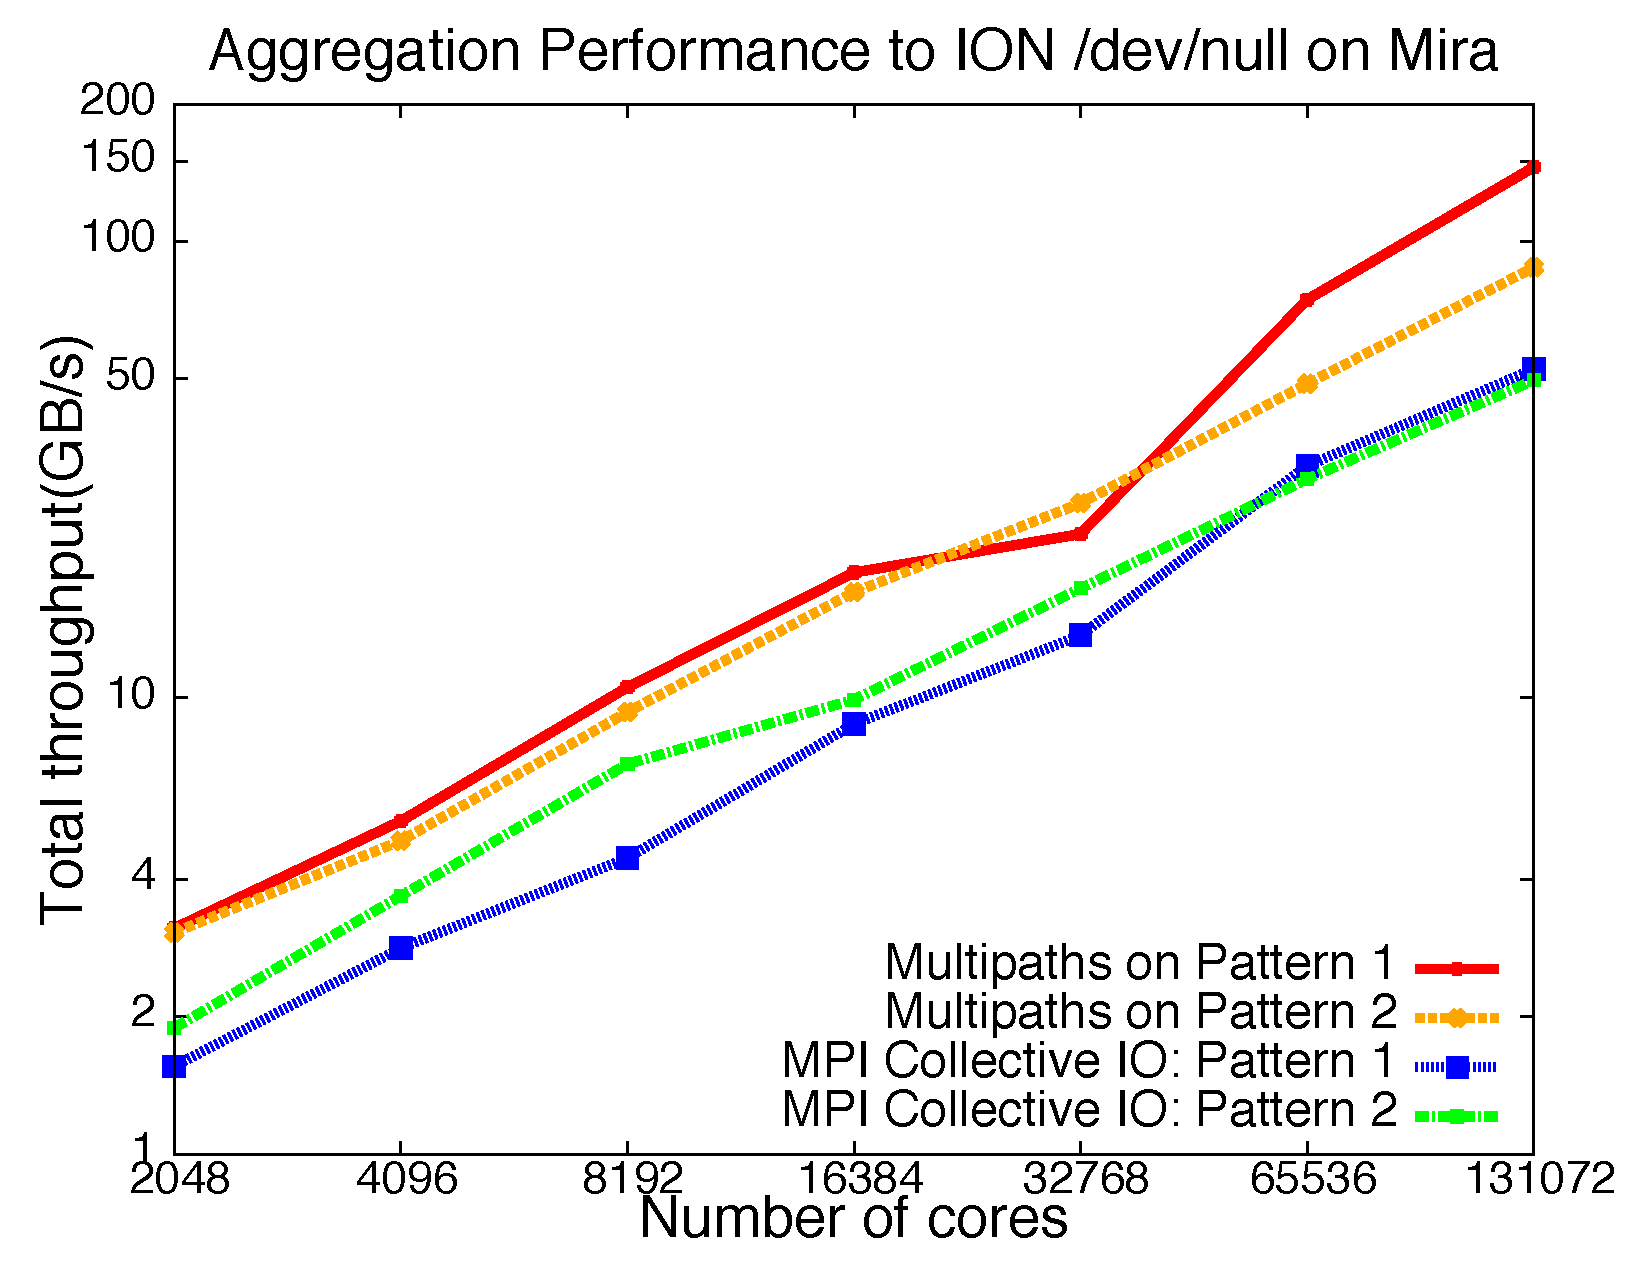
\includegraphics[scale=0.3]{mira_agg.pdf}
\caption{Efficacy of the approaches to move the data to /dev/null on the I/O nodes}
\label{fig:mira_agg}
\end{figure}

Figure \ref{fig:mira_agg} depicts the performance of our topology-aware multipath data movement approach in comparison with the default MPI-I/O for the two sparse data patterns as we scale from 2,048 cores to 131,072 cores on the Mira BG/Q system. On Pattern 1 (uniformly distributed data), we observe a $2\times$ improvement at 2,048 cores. The performance increases as we scale, and we achieve up to $3\times$ at 131,072 cores. On Pattern 2 (Pareto distributed data), we gain $1.5\times$ improvement at 2,048 cores and $2\times$ improvement at 131,072 cores. In the default MPI collective I/O case, the data movement uses a single deterministic path from the compute node to the bridge node and is unable to fully exploit all the available paths in the 5D torus of BG/Q for sparse data. Thus, we observe that leveraging network interconnect topology and multiple paths plays an important role at small scale and is critical at large scale. With the increased use of in situ analysis for supercomputing,  sparse data patterns for I/O are becoming increasingly important, and our approaches help provide more insights for improved performance.

Figure \ref{fig:mira_file} depicts the end-to-end performance of our topology-aware multipath data movement approach in comparison to the default MPI-I/O for the two sparse data patterns as we scale from 2,048 cores to 131,072 cores on the Mira BG/Q system to write this data out to the GPFS storage system. For both patterns, we observe a $2\times$ improvement in performance at lower core counts and up to $5\times$ improvement as we scale to larger core counts to 128K cores. This is primarily due to the fact that our  multi-path fully exploits all the available network paths to the I/O nodes and hence the storage systems for sparse data movement wherein multiple resources are potentially idle as in the case of the default MPI-I/O; data is routed along a deterministic single path. Thus, we observe the benefits of our approaches at scale for end-to-end data movement to the storage system.

\begin{figure}[!htb]
\centering
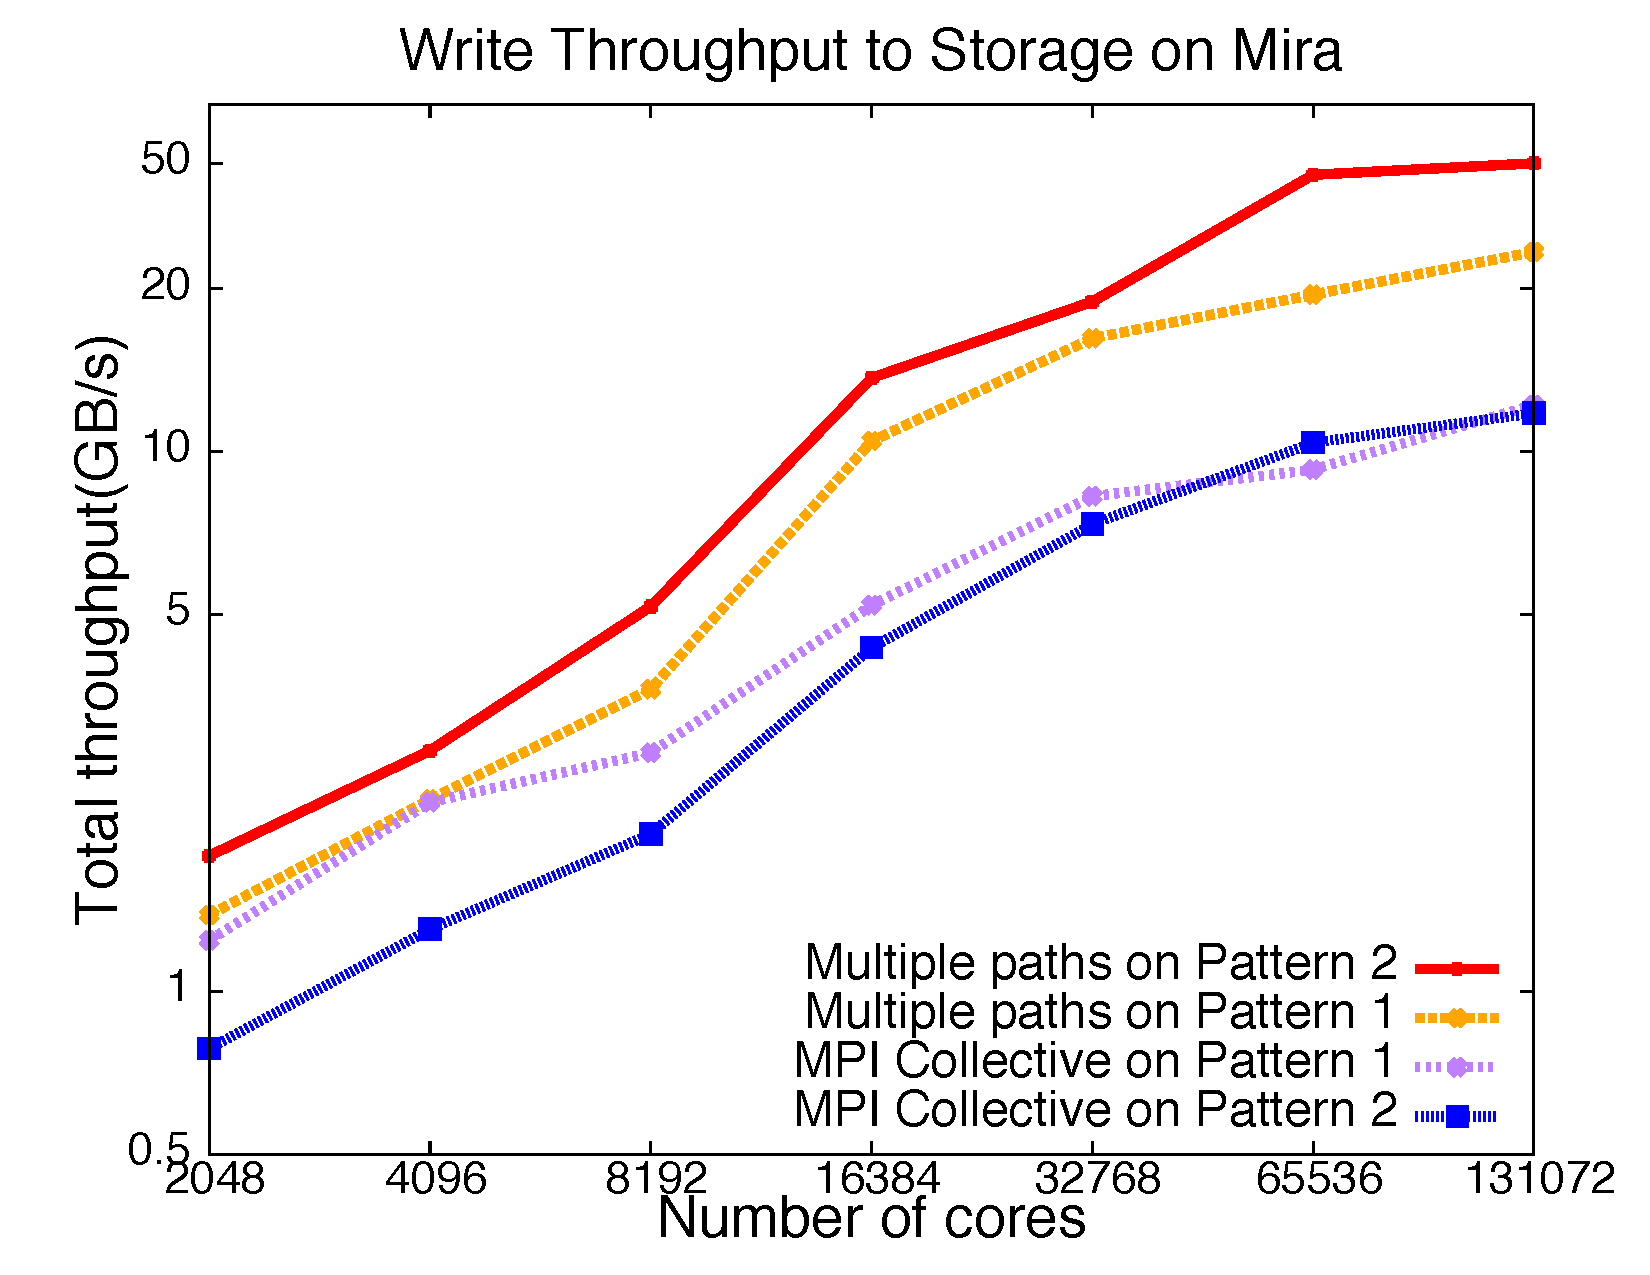
\includegraphics[scale=0.3]{mira_file.pdf}
\caption{End-to-end I/O throughput to the Mira GPFS parallel filesystem for the sparse patterns}
\label{fig:mira_file}
\end{figure}


\subsection{HACC I/O Application Benchmark}
HACC (Hardware/Hybrid Accelerated Cosmology Code) \cite{Habib:HACC} is a large-scale cosmology code suite that simulates the evolution of the universe through the first 13 billion years after the Big Bang. The simulation tracks the movement of trillions of particles as they collide and interact with each other, forming structures that transform into galaxies. During runtime, HACC writes data periodically to the storage system both for checkpoints and for I/O of the in situ analysis performed at simulation time. 
In this benchmark, we use HACC I/O, an I/O benchmark written to evaluate the performance of the I/O system for HACC.
We first evaluate the data movement performance from compute nodes to I/O nodes by writing to /dev/null. Next, we compare the end-to-end throughput of our mechanisms to default MPI collective I/O on HACC I/O to write the data to the GPFS parallel filesystem of Mira.  In this experiment, we scale our experiments from 2,048 up to 131,072 compute cores to simulate the collision of $768^3$ to $2,816^3$ particles. We write only 10\% of the generated data, which varies from 2 GB to 85 GB. The data is written from processes with MPI ranks within the range [4*num\_processes/10, 5*num\_processes/10], with the num\_processes being the total number of MPI ranks in our application. We collect the bandwidth information and report the average of 10 runs. Figure \ref{fig:hacc_file} depicts the achievable performance of writing the data to the GPFS parallel filesystem on Mira. 


From the figure we observe an overall improvement of 50\% throughput improvement for I/O. On GPFS, the locking overhead of the filesystem limits the achievable performance of a single shared file I/O. However, our multipath algorithm improves the overall data movement performance to the I/O node and hence improves the end-to-end performance. As a result of the in situ analysis, applications will tend to perform more I/O operations with significantly reduced data sizes. Thus multipath data movement will be of paramount importance for sparse I/O.


\begin{figure}[!htb]
\centering
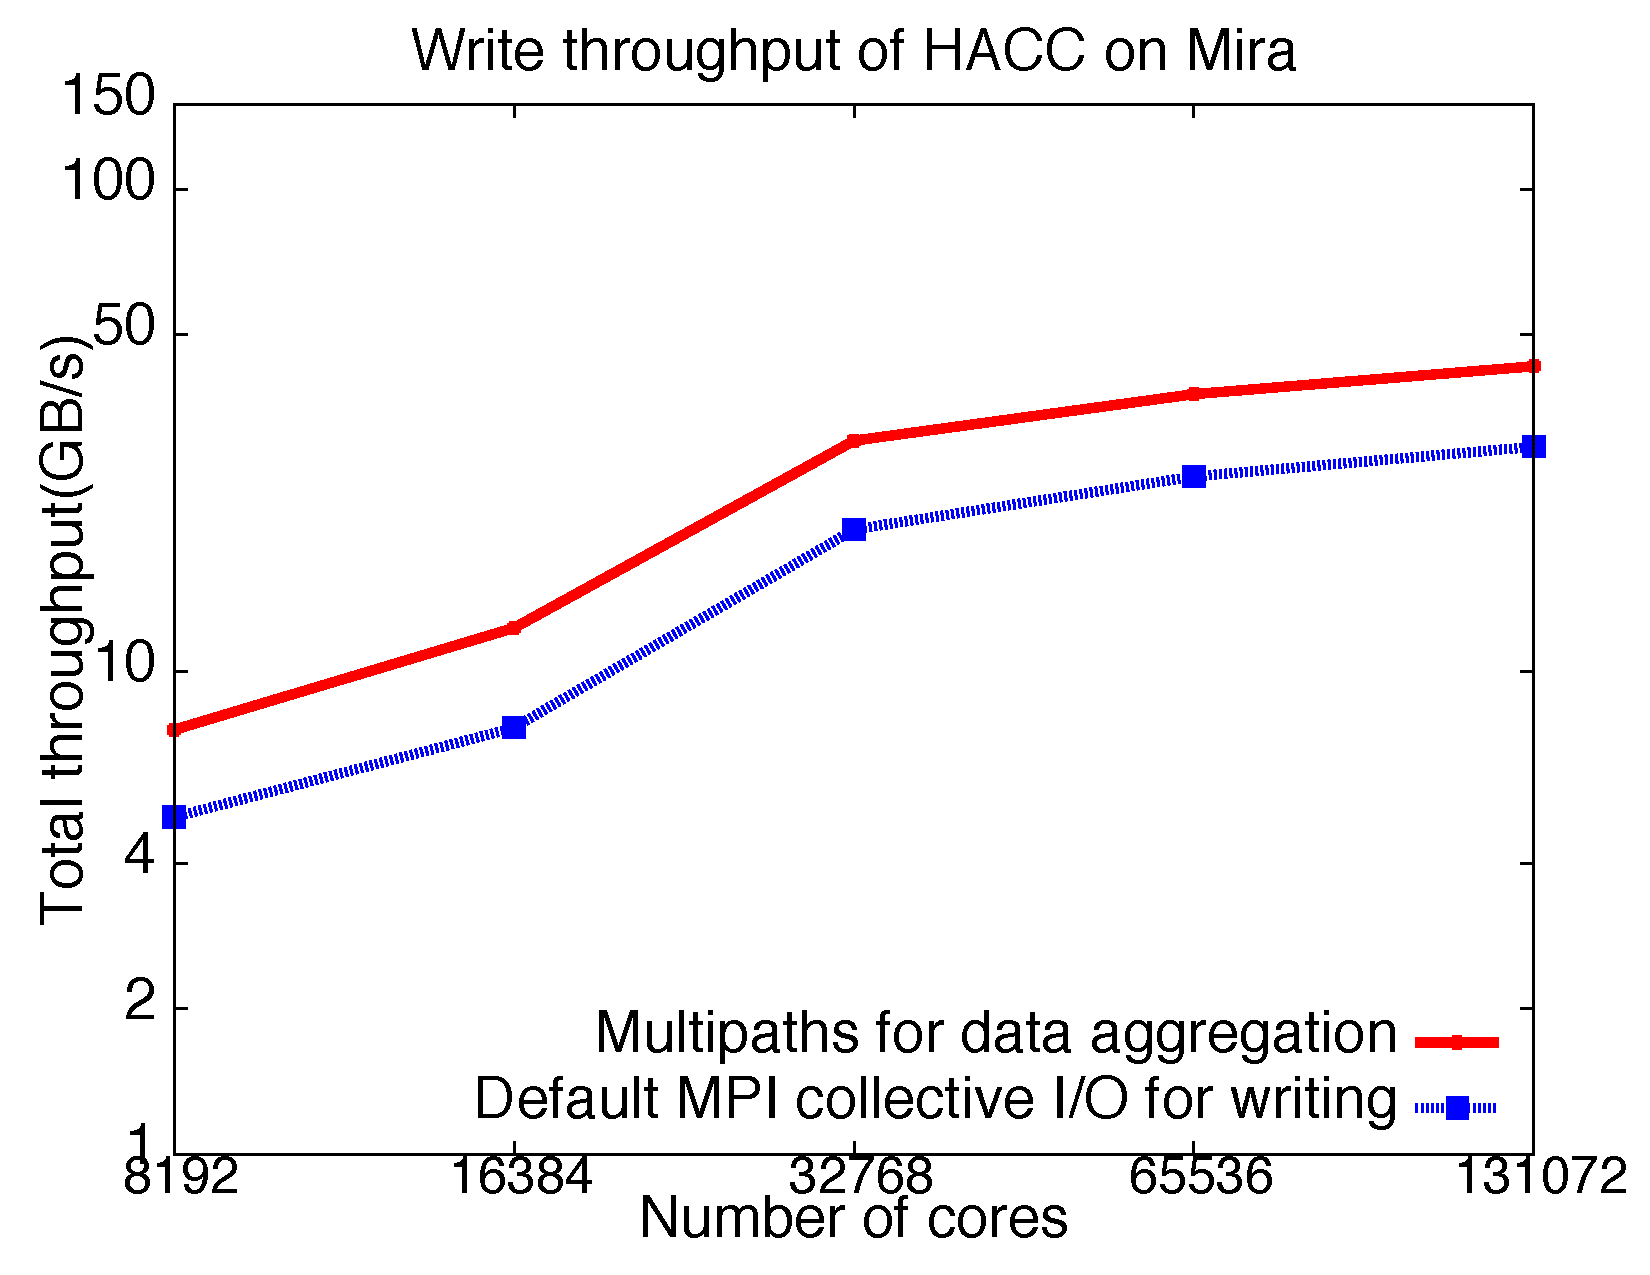
\includegraphics[scale=0.3]{hacc_agg.pdf}
\caption{End-to-end achievable throughput for in situ analysis of HACC I/O to Mira GPFS parallel filesystem }
\label{fig:hacc_file}
\end{figure}

\section{Conclusion} %and Future Work}
\label{sec:conclusion}
In this paper, we present our solution of using multipath data movement on leadership-class computer systems to improve the performance of sparse data movement. We present our graph models for different interconnect networks. We then use and enhanced Ford-Fulkerson algorithm to find the maximum flow and multiple paths, in order to gain the maximum flow in transferring data between two nodes or two groups of nodes. The data movement throughput is then improved further with pipelining techniques and using PAMI.  We demonstrate the efficacy of our solutions through a set of microbenchmarks and application benchmarks. On the Mira Blue Gene/Q system, we achieve up to $5\times$ improvement in performance for data movement using our approach for sparse data patterns.

%In future, we plan to work on adaptive routing at user space. When multiple paths are used, some may have longer paths with more proxies, or some may be in "hot-spot" communication of the systems, data size at source nodes may varied. In these cases, we need to route data dynamically and adaptively to gain stable performance improvement.

\section*{Acknowledgments}

This material is based upon work supported by the U.S. Department of Energy, Office of Science, under contract DE-AC02-06CH11357.
This research used resources of the Argonne Leadership Computing Facility (ALCF) at Argonne National Laboratory.
We thank the ALCF team for discussions and help related to this paper.

%% The Appendices part is started with the command \appendix;
%% appendix sections are then done as normal sections
%% \appendix

%% \section{}
%% \label{}

\section*{References}

%% If you have bibdatabase file and want bibtex to generate the
%% bibitems, please use
%%
\bibliographystyle{elsarticle-num} 
\bibliography{ref}

%% else use the following coding to input the bibitems directly in the
%% TeX file.

%\begin{thebibliography}{00}

%% \bibitem{label}
%% Text of bibliographic item

%% \bibitem{}

%\end{thebibliography}
\end{document}
\endinput
%%
%% End of file `elsarticle-template-num.tex'.
